% 编码：UTF-8。依据用户提供的“附件2 全文模板.docx”对齐会议全文格式。
\documentclass[UTF8,a4paper,twoside,zihao=5,fontset=windows]{ctexart}
\usepackage[left=23mm,right=23mm,top=28mm,bottom=25.4mm,headheight=12pt,headsep=5mm,footskip=10mm]{geometry}
\usepackage{amsmath,amssymb}
\usepackage{graphicx}
\usepackage{booktabs}
\usepackage{array}
\usepackage{placeins}
\usepackage{fancyhdr}
\usepackage{caption}
\setcounter{secnumdepth}{3}
\usepackage[hyperfootnotes=false,hidelinks]{hyperref}
\setmainfont{Times New Roman}
\setlength{\parskip}{0pt}
\setlength{\parindent}{2em}
% 五号正文、常规行距约 17 磅；含高公式的行按实际高度扩展。
\renewcommand{\baselinestretch}{1.35}
\ctexset{
    section={format=\raggedright\songti\zihao{4},aftername=\hspace{1em},beforeskip=8.5pt,afterskip=8.5pt},
    subsection={format=\raggedright\heiti\zihao{5},aftername=\hspace{1em},beforeskip=10pt,afterskip=4pt},
    subsubsection={format=\raggedright\songti\zihao{5},aftername=\hspace{1em},beforeskip=8pt,afterskip=4pt}
}
\pagestyle{fancy}
\fancyhf{}
% 模板采用奇偶页页眉；首页居中会议名，其余页码置于页眉外侧。
\fancyhead[LO,RE]{\songti\fontsize{7.5pt}{12pt}\selectfont 第七届新概念及高性能船学术研讨会}
\fancyhead[LE,RO]{\rmfamily\fontsize{7.5pt}{12pt}\selectfont\thepage}
\renewcommand{\headrulewidth}{0.75pt}
\renewcommand{\footrulewidth}{0pt}
\fancypagestyle{firstpage}{
    \fancyhf{}
    \fancyhead[C]{\songti\fontsize{7.5pt}{12pt}\selectfont 第七届新概念及高性能船学术研讨会}
    \renewcommand{\headrulewidth}{0.75pt}
}
\setlength{\heavyrulewidth}{1pt}
\setlength{\lightrulewidth}{0.5pt}
\makeatletter
\renewcommand{\tagform@}[1]{\maketag@@@{（\ignorespaces#1\unskip\@@italiccorr）}}
\renewcommand{\@makefntext}[1]{\parindent=2em\noindent\hspace{2em}\@makefnmark #1}
\makeatother
\newcommand{\templatefootnotesize}{\renewcommand{\baselinestretch}{1}\songti\fontsize{7.5pt}{10pt}\selectfont}
\let\footnotesize\templatefootnotesize
\captionsetup{font=small,labelsep=space,justification=centering,singlelinecheck=false,skip=4pt}
\newenvironment{conferenceabstract}{\par\begingroup\renewcommand{\baselinestretch}{1}\fangsong\fontsize{9pt}{17pt}\selectfont\setlength{\leftskip}{2em}\setlength{\rightskip}{2em}\setlength{\parindent}{2em}}{\par\endgroup}
\newcommand{\todo}[1]{\par\noindent{\songti【待撰写：#1】}\par}
% 逻辑冲突占位：代码实现存在矛盾、需修改代码后才能回填的内容。
\newcommand{\needfix}[1]{\par\noindent{\songti【需裁决：#1】}\par}

\title{考虑船桨匹配的翼帆助推船舶航程节油评估方法}
\author{作者姓名（待填写）\\单位名称（待填写）}
\date{}

\begin{document}
\setcounter{section}{-1}
\thispagestyle{firstpage}
\begin{center}
\vspace*{8pt}
{\heiti\fontsize{22pt}{28pt}\selectfont 考虑船桨匹配的翼帆助推船舶航程节油评估方法\par}
\vspace{12pt}
{\kaishu\fontsize{12pt}{17pt}\selectfont 作者姓名（待填写）\par}
\vspace{5pt}
{\kaishu\fontsize{9pt}{17pt}\selectfont（单位名称，城市 邮政编码，待填写）\par}
\end{center}
\vspace{8pt}

\begin{center}{\heiti\zihao{-4}摘\quad 要}\end{center}
\begin{conferenceabstract}
论文针对航运业节能减排需求，开发风帆助推船节能计算软件SailWing，并建立面向实际航线的船舶风帆助推能效分析方法。首先，基于船舶实际航迹开展航段划分与航迹特征提取，结合ERA5等气象数据对航行过程中的风速、风向等环境参数进行时空匹配，并通过气象聚类提取典型航行气象条件，为风帆性能及节能效果计算提供环境输入。在此基础上，针对翼帆、转筒帆建立相应气动性能计算模型。再进一步建立船体阻力、螺旋桨性能及燃油消耗计算模块，引入船桨相互作用参数，形成“阻力—螺旋桨—油耗”计算链路，并耦合风帆助推力开展船机桨帆匹配及节能效果分析。研究可为不同航线及气象条件下的风帆选型、运行参数优化和船舶绿色航行提供计算依据。
\par\noindent\textnormal{关键词：}\quad 翼帆助推；船桨匹配；航线风场；燃油消耗；节能评估
\par\noindent 中图分类号：待填写\hfill 文献标志码：A
\end{conferenceabstract}
\begingroup\renewcommand{\thefootnote}{}\footnotetext{基金项目：待填写（无基金资助时删除此项）。}\endgroup

\vspace{14pt}
\begin{center}
{\bfseries\fontsize{16pt}{23pt}\selectfont A voyage fuel-saving assessment method for wing-sail-assisted ships considering hull--propeller matching\par}
\vspace{5pt}
{\fontsize{12pt}{17pt}\selectfont Author Name (to be completed)\par}
\vspace{3pt}
{\zihao{-5}Affiliation, City, Postal Code, Country (to be completed)\par}
\end{center}
\vspace{7pt}
\begin{center}\textbf{Abstract}\end{center}
\begingroup\renewcommand{\baselinestretch}{1}\fontsize{10.5pt}{17pt}\selectfont\setlength{\parindent}{2em}
To address the need for energy conservation and emission reduction in the shipping industry, this study develops SailWing, a software tool for evaluating the energy-saving performance of wind-assisted ships, and establishes an energy-efficiency analysis method for actual shipping routes. First, actual vessel trajectories are segmented and their characteristics are extracted. Environmental parameters, including wind speed and direction, are matched to the trajectories in space and time using ERA5 and other meteorological datasets. Meteorological clustering is then applied to identify representative conditions, providing environmental inputs for sail performance and energy-saving calculations. Aerodynamic models are subsequently established for wing sails and Flettner rotors. Hull resistance, propeller performance, and fuel consumption modules are integrated with hull--propeller interaction parameters to form a resistance--propeller--fuel consumption calculation framework. Sail thrust is coupled with this framework to analyze the matching of the hull, engine, propeller, and sails and evaluate the resulting energy savings. The proposed method provides a computational basis for sail selection, operating parameter optimization, and environmentally sustainable ship operation under different route and meteorological conditions.
\par\textbf{Key words:}\quad wing-sail assistance; hull--propeller matching; route wind fields; fuel consumption; energy-saving assessment
\par\endgroup

\section*{作者简介}
{\renewcommand{\baselinestretch}{1}\songti\fontsize{9pt}{17pt}\selectfont\noindent 作者姓名：待填写；学历或职称、研究方向：待填写。\par\noindent 通讯作者：待填写。\par}

\section{引言}

风帆助推具有悠久的历史。虽然如今主机已被广泛运用于各种船上，但随着环境问题的不断加重，绿色环保理念的普及，风帆这一古老的助推方式重又被工程师带到实际工程上，重新焕发出新的生机。

根据风帆的形状和原理，还可以分为风筝帆、翼帆、转筒帆等。风筝帆又称天帆，受风筝空气动力学的启发而生。比起传统风帆，天帆系统每平方米产生的推进功率是传统风帆的六倍；值得一提的是，当主机出现故障时，牵引风帆可以作为船舶应急推进动力，降低船舶航行过程中机损的风险，从而提高船舶航行的安全性。当然，当遇到逆风或船行速度超过一定速度时，天帆系统将无法发挥作用。2007年，“天帆”公司研发制造了“白鲸天帆号”（图\ref{fig:intro-beluga}），用一张面积大概为160平方米的超轻合成纤维帆布，制成了一个外形类似于风筝的双层可充气风帆，利用电动桅杆放飞在货轮外，把它像风筝一样“放飞”到100—300米的空中，靠风力为船只提供辅助动力。“天帆系统”油耗节省率就可在10\%到35\%之间浮动，风力最理想时甚至可以短期节油50\%。

\begin{figure}[htbp]
\centering
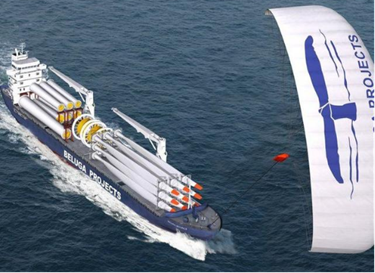
\includegraphics[width=0.70\textwidth,height=0.24\textheight,keepaspectratio]{figures/intro-beluga.png}
\caption{白鲸天帆号}
\label{fig:intro-beluga}
\end{figure}

船用翼帆一般指的是船上出于节能目的装设的、直接借助海上风能产生推进力的机翼形风帆，一般包括风帆结构、操帆装置、操帆装置控制系统、帆/桨联合控制系统等。2018年11月13日由中国船舶集团旗下大船集团为招商轮船建造全球首艘安装翼型帆装置的30.8万吨超大型原油船（VLCC）“凱力”号成功交付，充分证明了翼型帆方案在超大型船舶节能减排方面的有效性，标志着我国在船舶风力资源推广应用方面取得重大进展。除此之外，瑞典造船厂Wallenius Marine设计打造了一款可运载6000—7000辆小汽车的大型滚装帆船Oceanbird（图\ref{fig:intro-oceanbird}），其长200米，宽40米，高100米，载重吨位为32000吨，有望成为全球最大风帆动力货船。Oceanbird的动力几乎完全依靠风力，但也搭载了辅助电动机以应对进出港及紧急情况。凭借船上五片80米高的翼帆，Oceanbird可减少90\%的排放，对于减碳节能事业的发展都大有裨益。

\begin{figure}[htbp]
\centering
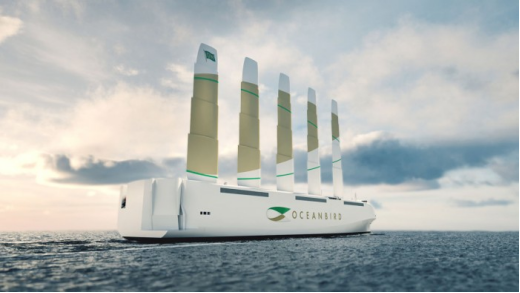
\includegraphics[width=0.70\textwidth,height=0.24\textheight,keepaspectratio]{figures/intro-oceanbird.png}
\caption{大型滚装帆船Oceanbird号}
\label{fig:intro-oceanbird}
\end{figure}

转筒帆技术，亦称为“福莱特转筒”（Flettner Rotor），是一种依靠“马格努斯效应”产生推进力的风力助推系统。转筒帆的工作原理是通过电机驱动垂直安装在甲板上的转筒旋转，当风吹过旋转的转筒时，空气动力学效应产生推力。这种技术的特点在于其在各种风向条件下均能提供稳定的辅助动力。2024年，全球领先的大型船用机械风帆供应商Norsepower，宣布与Union Maritime Limited签署了一项合作协议，为其全新成品油轮船队配备Norsepower Rotor Sails（挪世航力旋筒风帆），如图\ref{fig:intro-norsepower}所示。本次交易内容包含为四艘由我国福建东南造船有限公司和芜湖造船厂有限公司建造的新造船装配旋筒风帆，另外八艘船舶也将采用旋筒风帆，便于后期加装。

\begin{figure}[htbp]
\centering
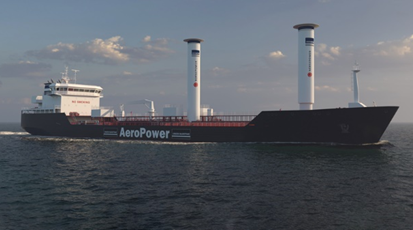
\includegraphics[width=0.70\textwidth,height=0.24\textheight,keepaspectratio]{figures/intro-norsepower.png}
\caption{配备两台挪世航力旋筒风帆的化学品油轮}
\label{fig:intro-norsepower}
\end{figure}

这些企业所开发的风力辅助推进技术已经在商业航运领域获得了实质性的应用与验证。它们被广泛应用于各类船舶，包括货轮、客轮、油轮等，且在多样化的航线和航行条件下经历了严格的测试与实际运营。这些技术显著提升了船舶的能源效率和环保性能，有效降低了燃料消耗及碳排放。

尽管如此，风力辅助推进技术的商业化及其在更广泛领域的应用仍面临诸多挑战。风帆的安装和使用仍然需要依据船舶个性化定制、风帆对船舶的性能影响仍缺乏系统研究。针对该问题，劳氏船级社开发的 Flettner 转筒帆节油计算器可针对不同船型、航线及季节条件评估转筒帆的节油潜力，并考虑螺旋桨性能、主机负荷相关燃油消耗率及转筒驱动能耗，为风力助推装置的初步评估提供了工具基础\textsuperscript{\cite{lr2021flettner}}。

面向实际航行过程中的环境差异及不同风帆形式的分析需求，本文开发风帆助推船节能计算软件 SailWing，依托课题组翼型帆、转筒帆等研究基础，整合实船基础参数、航行数据等，优化风帆—实船一体化能效计算模型，并建立程序评估典型风帆的节能效果，量化不同风帆配置、风场条件下的实船能耗与节能效率。重点开展以下研究：基于实际航迹匹配 ERA5 等气象数据，采用 K-means 聚类提取典型航行气象工况，并结合航迹特征开展航段划分，为航线能效分析提供环境输入；支持翼帆与转筒帆的气动性能计算，为不同风帆助推形式的方案比较提供工具；提供螺旋桨敞水数据导入、已知几何参数性能计算和设计点匹配三种方式，分别求解有帆与无帆工况下的螺旋桨工作点，并结合负荷相关燃油消耗率计算航程油耗。本文的研究贡献主要体现在增加多种帆型和航线的选择，根据航线气象条件实现不同风帆的实时推力分析，考虑船机桨帆的匹配，对船上不同风帆安装位置、不同风帆数量、不同船舶参数、不同船舶航线进行节能效果的评估，展示在航线上各航段的节省燃油或CO$_2$排放上的收益。

\FloatBarrier

\section{翼帆助推船舶节油评估模型}
\subsection{实际航线气象环境提取与典型气象工况划分}
\label{sec:meteo}

风帆助推效果取决于船舶航行过程中遭遇的风、浪、流条件。针对再分析环境场与航迹点在
时空尺度上的不一致，首先将环境资料匹配至实际航迹；在此基础上识别航行过程中具有
代表性的环境状态；进而结合气象状态连续性与航迹几何特征确定航段边界，
形成面向后续能效分析的航段环境输入。

\subsubsection{数据来源与环境变量}

风、浪资料取自 ERA5 再分析产品，海流资料取自 CMEMS 全球海洋再分析产品 GLORYS12V1，
所选变量及其在后续计算中的作用见表~\ref{tab:meteo_sources}。

\begin{table}[htbp]
\centering
\small
\setlength{\tabcolsep}{4pt}
\renewcommand{\arraystretch}{1.4}
\caption{气象数据来源、变量与研究中的作用}
{\small Table~\thetable\quad Meteorological data sources, variables and their roles in this study\par}
\smallskip
\label{tab:meteo_sources}
\begin{tabular}{@{}>{\raggedright\arraybackslash}p{1.5cm}>{\raggedright\arraybackslash}p{2.1cm}>{\raggedright\arraybackslash}p{2.8cm}>{\raggedright\arraybackslash}p{2.05cm}>{\raggedright\arraybackslash}p{5.4cm}@{}}
\toprule
数据源 & 变量（本文符号） & 物理含义 & 空间/时间分辨率 & 在研究中的作用 \\
\midrule
ERA5 & \texttt{u10}、\texttt{v10} & 10 m 风的东西/南北分量 & 0.25\textdegree{} / 1 h & 风速与风向，风帆气动计算的来流条件 \\
ERA5 & \texttt{swh} & 有效波高 & 0.50\textdegree{} / 1 h & 波浪环境分类及后续阻力修正输入 \\
ERA5 & \texttt{mwd}、\texttt{mwp} & 平均波向、平均波周期 & 0.50\textdegree{} / 1 h & 波浪环境 \\
CMEMS & \texttt{uo}、\texttt{vo} & 表层海流东西/南北分量 & 1/12\textdegree{} / 1 d & 海流环境分类及后续航速修正输入 \\
\bottomrule
\end{tabular}
\end{table}
\FloatBarrier

方向角采用以正北为 0\textdegree{}、顺时针为正的定义，风向与流向由其东西向、南北向速度分量
反算得到，表示相应速度矢量的指向，与气象学中表示风来向的定义相差 180\textdegree{}。
ERA5 波向 \texttt{mwd} 的方向定义依据产品文档进一步确认【待确认】，
在确认之前不将其与风向进行直接角度比较。

算例选取 2024 年 5 月、120\textdegree{}～128\textdegree{}E、36\textdegree{}～38\textdegree{}N 海域的环境资料，共 744 个时刻。
风场、波浪和海流数据的缺测率分别为 0\%、32.9\% 和 34.7\%，
其中波浪和海流的缺测主要对应陆地区域掩膜。此外，建立了支持全球全年数据下载、
分块归档及断点续传的数据处理框架，全球全年数据的统计分析不属于本文研究范围【待填】。

\subsubsection{航迹与气象环境的时空匹配}

再分析环境资料在时间分辨率与空间网格上均与航迹点不一致：风、浪为逐小时序列，
海流为日均值；风、浪、流网格分辨率分别为 0.25\textdegree{}、0.50\textdegree{} 与 1/12\textdegree{}，
而航迹点为任意时空位置的离散采样。因此采用时间线性插值与空间双线性插值相结合的
方法，将 \texttt{u10}、\texttt{v10}、\texttt{swh}、\texttt{mwd}、\texttt{mwp}、\texttt{uo}、\texttt{vo} 匹配至各航迹点。
该方法在相邻网格内环境场连续变化的假设下可降低网格离散引起的空间跳变，
其精度受再分析资料自身精度制约；本文未将插值结果与现场实测环境作真值比对。

航迹侧处理包括两项：以出发点经纬度与出发时刻为基准平移航迹时间轴，
使航迹与环境资料处于同一时段；对跨越 ±180\textdegree{} 的航迹进行经度展开，
避免经度差出现约 360\textdegree{} 的虚假跳跃。

海流数据为日均值，采用对应日期的日均流场表征航迹时刻的背景流动条件。

经上述处理，2024 年 5 月 7 日去程算例共获得 \textbf{813 个有效航迹点}，
作为后续聚类与航段划分的样本。

\subsubsection{气象特征构造与标准化}

以航迹点对应的环境状态为聚类对象，由风、浪、流要素构造 10 维特征向量，
包括风速、风向（正弦、余弦编码）、波向（正弦、余弦编码）、有效波高、波周期、
流速及流向（正弦、余弦编码）。

由于方向变量具有周期性，直接采用角度数值计算欧氏距离会在 0\textdegree{}/360\textdegree{} 附近产生不连续，
因此采用正弦、余弦双变量编码，两点的编码距离为

\begin{equation}
\begin{aligned}
d_\theta&=\sqrt{(\sin\theta_1-\sin\theta_2)^2+(\cos\theta_1-\cos\theta_2)^2}\\
&=2\left|\sin\frac{\Delta\theta}{2}\right|.
\end{aligned}
\label{eq:meteo_direction_distance}
\end{equation}

当角差较小时，式\eqref{eq:meteo_direction_distance}与真实角差成正比，可保持方向量的周期性。

各特征量纲不同，为消除量纲影响，按全部样本对特征作全局标准化，
使不同航段的代表状态位于同一尺度上：
\begin{equation}
z_{ij}=\frac{x_{ij}-\mu_j}{\sigma_j}.
\label{eq:meteo_standardization}
\end{equation}
式中，$\mu_j$ 和 $\sigma_j$ 分别为第 $j$ 维特征在全部样本中的均值和标准差。在此基础上可对特征施加权重，
以反映各环境要素的相对重要性；基准算例采用等权设置，
加权方案用于评价特征重要性设定对聚类结果的影响（见本节特征权重敏感性分析）。
航段工况赋值采用与聚类阶段一致的标准化参数及特征权重，以使两阶段处于统一的特征空间。

\subsubsection{典型气象工况聚类}

\par\noindent\textbf{聚类方法与簇数确定}

聚类采用 KMeans 方法，在标准化特征空间中最小化簇内平方和

\begin{equation}
\mathcal{J}=\sum_{c=1}^{k}\sum_{\boldsymbol{z}_i\in C_c}
\left\|\boldsymbol{z}_i-\boldsymbol{\mu}_c\right\|^2.
\label{eq:meteo_kmeans_objective}
\end{equation}

考虑不同簇数对工况分辨率及聚类稳定性的影响，在 k = 2～8 范围内进行对比，
并采用簇内平方和、轮廓系数、Calinski–Harabasz（CH）指数及 Davies–Bouldin（DB）指数
综合评价聚类效果，结果见表~\ref{tab:meteo_cluster_numbers}。其中轮廓系数与 CH 指数越大、DB 指数越小，
表示聚类效果越好。

\begin{table}[htbp]
\centering
\small
\setlength{\tabcolsep}{4pt}
\renewcommand{\arraystretch}{1.4}
\caption{簇数评价结果（813 个航迹点，等权方案）}
{\small Table~\thetable\quad Evaluation of cluster numbers (813 trajectory points, equal-weight scheme)\par}
\smallskip
\label{tab:meteo_cluster_numbers}
\begin{tabular}{@{}rrrrr@{}}
\toprule
k & 簇内平方和 & 轮廓系数 & CH 指数 & DB 指数 \\
\midrule
2 & 3816.63 & 0.5148 & 916.55 & 0.8048 \\
\textbf{3} & \textbf{1989.28} & \textbf{0.5491} & \textbf{1250.19} & \textbf{0.7134} \\
4 & 1625.14 & 0.5151 & 1079.38 & 0.8991 \\
5 & 1324.72 & 0.4668 & 1037.71 & 0.9486 \\
6 & 1087.03 & 0.4658 & 1045.72 & 0.8680 \\
7 & 886.93 & 0.4887 & 1097.03 & 0.7426 \\
8 & 746.67 & 0.4756 & 1137.16 & 0.7959 \\
\bottomrule
\end{tabular}
\end{table}
\FloatBarrier

由表~\ref{tab:meteo_cluster_numbers} 可知，k = 3 时轮廓系数和 CH 指数达到最大值，同时 DB 指数取得最小值，
三项评价指标均支持 k = 3，因此等权特征方案下取 k = 3 作为基准聚类结果。

\par\noindent\textbf{聚类结果}

3 类典型气象工况的代表值及样本数见表~\ref{tab:meteo_conditions}。

\begin{table}[htbp]
\centering
\small
\setlength{\tabcolsep}{4pt}
\renewcommand{\arraystretch}{1.4}
\caption{本航次典型气象工况（2024 年 5 月 7 日去程，k = 3）}
{\small Table~\thetable\quad Typical meteorological conditions of this voyage (outbound, 2024-05-07, k = 3)\par}
\smallskip
\label{tab:meteo_conditions}
\textbf{（a）样本分布与风场特征}\par\smallskip
\begin{tabular}{@{}lrrrr@{}}
\toprule
工况 & 样本数 & 占比 & 风速 (m/s) & 风向 (°) \\
\midrule
簇 0 & 255 & 31.4\% & 3.60 & 195.9 \\
簇 1 & 312 & 38.4\% & 2.82 & 97.0 \\
簇 2 & 246 & 30.3\% & 5.77 & 232.5 \\
\bottomrule
\end{tabular}\par\medskip\textbf{（b）波浪与海流特征}\par\smallskip
\begin{tabular}{@{}lrrrrr@{}}
\toprule
工况 & 有效波高 (m) & 波向 (°) & 波周期 (s) & 流速 (m/s) & 流向 (°) \\
\midrule
簇 0 & 0.54 & 354.4 & 4.21 & 0.05 & 31.0 \\
簇 1 & 0.51 & 3.9 & 4.27 & 0.12 & 116.6 \\
簇 2 & 0.42 & 44.7 & 2.88 & 0.03 & 259.8 \\
\bottomrule
\end{tabular}
\end{table}
\FloatBarrier

3 类工况的主要差异表现为风速及风向组合的变化。簇 2 具有最高的平均风速，
但其有效波高和波周期均低于簇 0 和簇 1，表明该航次中风场强度与局地波浪状态
并未呈现简单的一一对应关系。该差异可能与波浪的演化及传播过程有关，
但仅依据当前航次数据尚无法进一步判定其具体机制。

\par\noindent\textbf{特征权重敏感性}

为评价聚类结果对特征重要性设定的敏感程度，构建 5 组特征权重方案并分别确定
其最优簇数，结果见表~\ref{tab:meteo_weights}。

\begin{table}[htbp]
\centering
\small
\setlength{\tabcolsep}{4pt}
\renewcommand{\arraystretch}{1.4}
\caption{特征权重方案的敏感性（813 个航迹点）}
{\small Table~\thetable\quad Sensitivity of the clustering result to feature weights (813 trajectory points)\par}
\smallskip
\label{tab:meteo_weights}
\begin{tabular}{@{}lrrrr@{}}
\toprule
权重方案 & 最优 k & 轮廓系数 & CH 指数 & DB 指数 \\
\midrule
等权（基准） & 3 & 0.549 & 1250.2 & 0.713 \\
风主导 & 3 & 0.569 & 1467.5 & 0.685 \\
风浪并重 & 8 & 0.526 & 1863.3 & 0.662 \\
波浪主导 & 2 & 0.629 & 1785.6 & 0.582 \\
忽略海流 & 8 & 0.550 & 2154.7 & 0.623 \\
\bottomrule
\end{tabular}
\end{table}
\FloatBarrier

由表~\ref{tab:meteo_weights} 可知，提高波浪要素权重后簇结构的可分性指标有所改善，
但对应的最优簇数由 k = 3 变为 k = 2，表明聚类结构与最优簇数受特征权重影响。
考虑到后续能效分析对环境工况分辨能力的要求，将等权方案下的 k = 3
作为后续航段划分与能效分析的基准工况设置，其余权重方案用于评价聚类结果
对特征重要性设定的敏感程度。

\subsubsection{气象工况驱动的航段划分}

气象工况聚类描述环境状态，航段划分描述空间连续的航行区间，两者属于不同层次的处理过程。
航段划分在工况识别结果的基础上进行：沿航线构造局部区间，
以区间内环境特征的均值表征该区间状态；依据该状态与各聚类中心的距离完成工况归属；
根据相邻区间工况状态的相似程度进行合并；将航迹转向点作为几何约束引入边界确定过程，
从而形成气象状态约束与航迹几何约束相结合的航段划分。

相邻区间的代表工况在标准化空间中的距离不超过合并阈值时，合并为同一航段。
合并阈值取聚类中心两两距离中位数与合并系数的乘积，本算例中位数与合并系数分别为
4.81 与 0.5，对应阈值为 2.403。

算例最终得到 7 个分割点与 6 个航段，航段划分结果见表~\ref{tab:meteo_segments}。

\begin{table}[htbp]
\centering
\small
\setlength{\tabcolsep}{4pt}
\renewcommand{\arraystretch}{1.4}
\caption{航段划分结果}
{\small Table~\thetable\quad Segmentation results of the voyage\par}
\smallskip
\label{tab:meteo_segments}
\begin{tabular}{@{}>{\raggedright\arraybackslash}p{0.8cm}>{\raggedright\arraybackslash}p{2.2cm}>{\raggedright\arraybackslash}p{2.2cm}>{\raggedright\arraybackslash}p{2.0cm}>{\raggedright\arraybackslash}p{2.6cm}>{\raggedright\arraybackslash}p{2.0cm}>{\raggedright\arraybackslash}p{1.15cm}@{}}
\toprule
航段 & 起点 & 终点 & 大圆距离/km & 平均航速/($\mathrm{m\,s^{-1}}$) & 平均航向/(°) & 所属工况 \\
\midrule
1 & 121.46\textdegree{}E\newline 37.60\textdegree{}N & 122.80\textdegree{}E\newline 37.65\textdegree{}N & 118.2 & 9.90 & 87.1 & 簇 1 \\
2 & 122.80\textdegree{}E\newline 37.65\textdegree{}N & 123.44\textdegree{}E\newline 37.44\textdegree{}N & 61.3 & 10.53 & 111.9 & 簇 1 \\
3 & 123.44\textdegree{}E\newline 37.44\textdegree{}N & 125.42\textdegree{}E\newline 37.09\textdegree{}N & 180.3 & 10.05 & 102.0 & 簇 0 \\
4 & 125.42\textdegree{}E\newline 37.09\textdegree{}N & 126.00\textdegree{}E\newline 36.99\textdegree{}N & 52.2 & 9.26 & 102.2 & 簇 2 \\
5 & 126.00\textdegree{}E\newline 36.99\textdegree{}N & 126.17\textdegree{}E\newline 37.02\textdegree{}N & 16.0 & 8.62 & 77.5 & 簇 2 \\
6 & 126.17\textdegree{}E\newline 37.02\textdegree{}N & 126.51\textdegree{}E\newline 37.35\textdegree{}N & 47.2 & 8.55 & 39.2 & 簇 2 \\
\bottomrule
\end{tabular}
\end{table}
\FloatBarrier

表~\ref{tab:meteo_segments} 中距离为相邻分割点之间的大圆距离，平均航速由该距离与对应航段时间间隔确定。
各航段的代表性环境参数取该航段所属工况的聚类中心（表~\ref{tab:meteo_conditions}），
因此 6 个航段对应 3 组环境条件：航段 1、2 属簇 1，航段 3 属簇 0，航段 4～6 属簇 2。
据此，每个航段可直接引用表~\ref{tab:meteo_conditions} 中对应工况的风速、风向、有效波高、波向、波周期、
流速与流向，以及由其反算的风、流速度分量，作为后续风帆气动计算与船机桨帆匹配的输入。

\subsubsection{讨论}

当前结果主要基于单一航次样本，所得工况用于表征该航次的环境状态，
不宜直接推广至全年航线。CMEMS 日均流场难以反映潮汐等高频流动过程，
再分析资料与现场实测之间的偏差也可能影响航迹点环境状态的匹配精度。
此外，ERA5 波向的方向定义尚待依据产品文档确认，
在此之前不对波向与风向的关系作进一步推断。后续可引入多航次、多季节实测航迹
及更高时空分辨率的海洋环境资料，对工况分类结果进行验证。

\subsubsection{小结}

本节建立了面向实际航线的气象环境提取与工况划分方法。通过再分析风、浪、流场与
AIS 航迹的时空匹配，构建包含风、浪、流特征的环境状态向量，并利用 KMeans
识别典型气象工况。在 2024 年 5 月 7 日去程航次算例中，等权方案下获得 3 类典型
环境状态，并进一步结合气象状态连续性与航迹几何特征划分为 6 个航段。
所得航段环境参数可为后续风帆气动性能计算及船机桨帆匹配提供输入。


\par\noindent\textbf{与推进模型的衔接}
本节波浪与海流参数用于环境状态分类，并为后续环境修正提供输入；第~\ref{sec:ship_propeller}~节采用静水阻力模型，尚未显式计入波浪附加阻力和海流修正。本节气象算例的平均航速随航段变化，而推进模型以定航速准稳态计算为基础，后续能效算例需统一航速定义及取值，并明确对地航速与对水航速的转换关系。
\par\noindent\textit{【待核实：补充 ERA5、CMEMS、KMeans 及轮廓系数、CH/DB 指数的正式参考文献。】}
\subsection{风帆气动力计算模型与计算流程}
\label{sec:sail_aero}

风帆产生的助推力取决于船舶航行中遭遇的表观风条件与风帆自身的气动特性。本节在统一的
坐标与来流定义下，分别建立翼帆与转筒帆的气动模型：翼帆采用二维翼型极线并经全攻角范围
扩展，转筒帆采用基于非定常 RANS 数值结果拟合的代理模型；进而给出升阻力到船舶纵向
助推力与侧向力的合成关系，并以纵向推力最大为目标确定各航路点的风帆工作点；最后给出
本节气动计算与后续推进计算的衔接流程。本节侧重模型建立与实现方式，算例分析、
参数影响与模型验证见第~3~章。

\subsubsection{坐标、来流与受力定义}

定义风翼受力分析所用的角度体系如图~\ref{fig:sail_force} 所示\textsuperscript{\cite{yanyasheng2019}}。以船舶航向为参考方向，
各角度定义如下：
\begin{itemize}
\item $\beta$ —— 相对风向角，船舶航向与实际风向的夹角；相对风的方向由
实际风向绕航向转过 $\beta$ 角得到；
\item $\alpha$ —— 风翼攻角，风翼弦线与相对风向的夹角；
\item $\varphi$ —— 风翼角，风翼弦线与船舶船向的夹角；
\item $\gamma$ —— 船舶漂角，船舶航向与船向的夹角。
\end{itemize}
本文以 $\varphi$ 表示风翼角。船体静力学中 $\varphi$ 常记为横倾角，本节不涉及横倾，
与后文可能出现的横倾符号不构成冲突。

\begin{figure}[htbp]
\centering
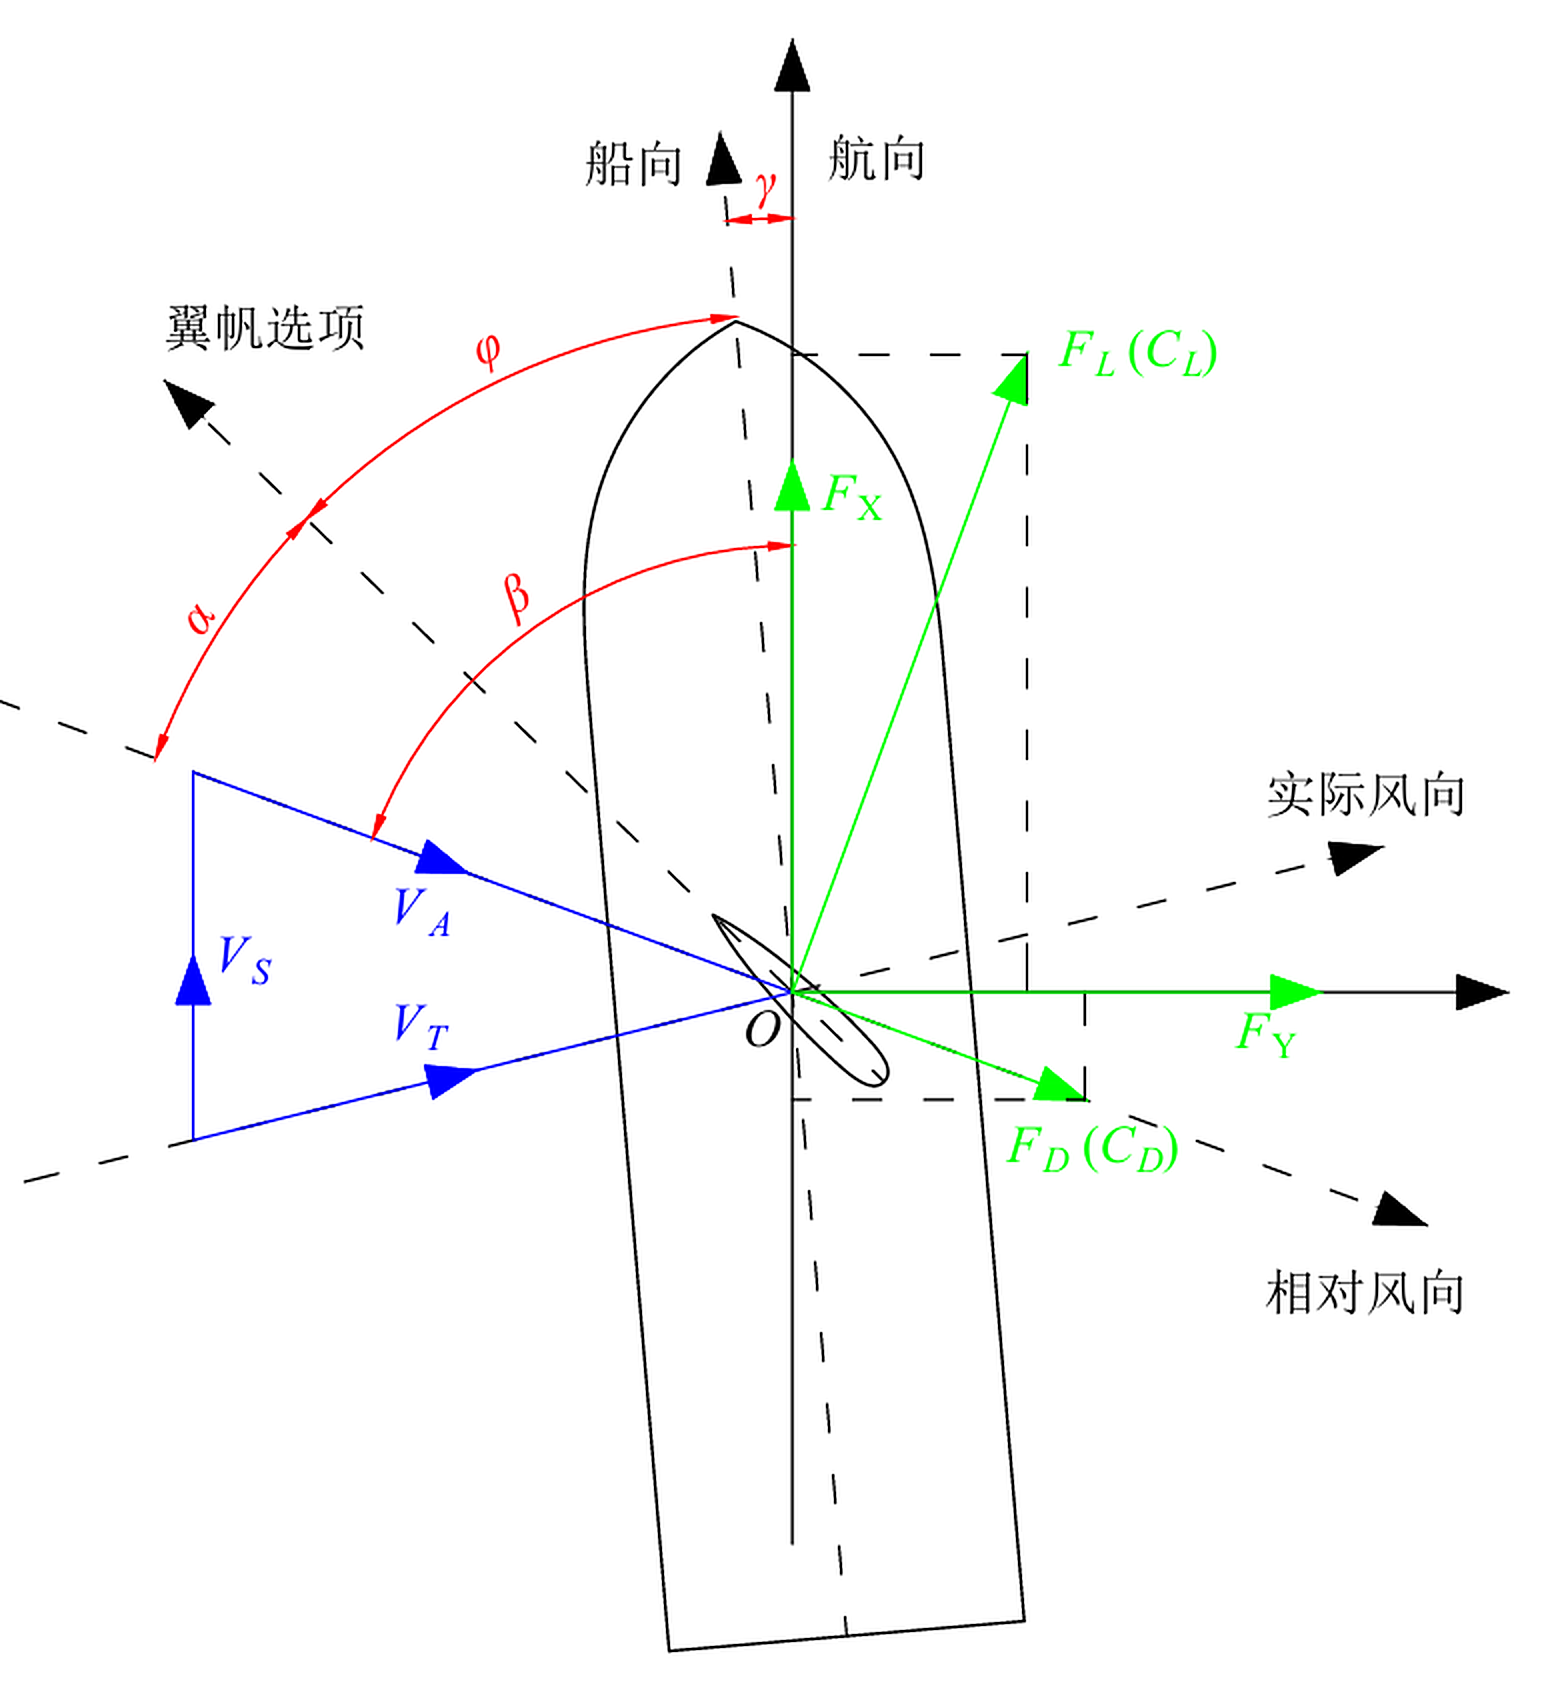
\includegraphics[width=0.68\textwidth]{figures/fig_1_2_force.png}
\caption{风翼受力简图（$\beta$、$\alpha$、$\varphi$ 为本文所用角度体系）}
{\small Fig.~\thefigure\quad Force diagram of a wing sail ($\beta$, $\alpha$ and $\varphi$ defined as in the text)\par}
\label{fig:sail_force}
\end{figure}
\FloatBarrier

船舶以航速 $V_s$ 航行时，相对风由真风 $V_T$ 与船速矢量合成，记为 $V_A$，其大小为
$v$。当相对风以攻角 $\alpha$ 吹向风翼时，垂直于相对风方向产生升力 $F_L$，沿相对风
方向产生阻力 $F_D$；升阻力在船舶航向上合成得到助推力 $F_T$，在垂直航向方向合成得到
侧推力 $F_S$。侧推力会使船舶偏航产生漂角，航行中需要依靠舵效矫正。升力、阻力与
风阻力矩 $M$ 分别表示为
\begin{equation}
F_L=\frac{1}{2}\rho v^2AC_L,\qquad
F_D=\frac{1}{2}\rho v^2AC_D,\qquad
M=\frac{1}{2}\rho v^2AlC_M,
\label{eq:lift_drag_moment}
\end{equation}
式中，$\rho$ 为空气密度；$v$ 为相对风速；$A$ 为风翼面积；$l$ 为参考弦长；
$C_L$、$C_D$、$C_M$ 分别为升力系数、阻力系数与风阻力矩系数。

气动系数是攻角与风翼几何参数的函数，一般形式为
\begin{equation}
C_L=f\!\left(\alpha,\lambda,\varepsilon\right),\quad
C_D=g\!\left(\alpha,\lambda,\varepsilon\right),\quad
C_M=h\!\left(\alpha,\lambda,\varepsilon,l\right),
\label{eq:coef_functions}
\end{equation}
式中，$\lambda$ 为风翼展弦比；$\varepsilon$ 为风翼拱度比。本文将风翼视为可绕垂直桅轴
旋转的对称翼型直翼，其气动特性由二维翼型极线 $C_L(\alpha)$、$C_D(\alpha)$ 与受风面积
表征，三维几何形状不进入气动力计算，仅用于程序中的模型显示。由此，风帆气动模型归结为
两个问题：一是获得翼帆与转筒帆的升阻力系数随其控制变量（翼帆为攻角 $\alpha$，
转筒帆为转筒比 $SR$）的变化关系，即气动极线；二是由极线确定各航路点的最优工作点。
二者分别由~\S\ref{sec:wing_polar}~与~\S\ref{sec:rotor_model}~、
\S\ref{sec:sail_operating_point}~给出。

计算雷诺数按设计航速与弦长估算：
\begin{equation}
Re=\frac{V_s c}{\nu_a},
\label{eq:wing_re}
\end{equation}
式中，$c$ 为翼帆弦长；$\nu_a=1.5\times10^{-5}\ \mathrm{m^2\,s^{-1}}$ 为常温下空气的
运动黏度。当航速或弦长缺失时取 $Re=1.0\times10^{6}$ 作为默认值。空气密度取
$\rho=1.225\ \mathrm{kg\,m^{-3}}$，马赫数取 0（不计压缩性）。

\subsubsection{翼帆气动模型}
\label{sec:wing_polar}

\paragraph{二维极线计算}
翼帆气动特性由翼型极线 $C_L(\alpha)$、$C_D(\alpha)$ 表征，采用 XFOIL 程序计算。
XFOIL 是针对低雷诺数翼型的黏性/无黏耦合分析程序\textsuperscript{\cite{drela1989}}，
通过全局牛顿迭代实现无黏流场、
边界层方程与转换模型的耦合求解，可在保证计算精度的前提下高效给出翼型压力分布、
升力系数、阻力系数与失速特性。程序中调用 XFOIL 的流程为：按标准格式写入翼型坐标
文件，生成批处理输入脚本，依次执行翼型载入、黏性分析开启、雷诺数与马赫数设定、
迭代上限设定、极线累加与攻角序列扫描，最后写出极线文件并解析。计算设置取马赫数为 0、
攻角区间为 $-15^{\circ}\sim15^{\circ}$、步长为 $1^{\circ}$、黏性迭代上限为 100。
极线文件按 XFOIL 标准列格式输出攻角、升力系数、阻力系数、压差阻力系数与俯仰力矩
系数；其中压差阻力系数与俯仰力矩系数暂不参与本文计算，保留以便后续扩展配平分析。
算例翼型的极线见图~\ref{fig:polar}。

\begin{figure}[htbp]
\centering
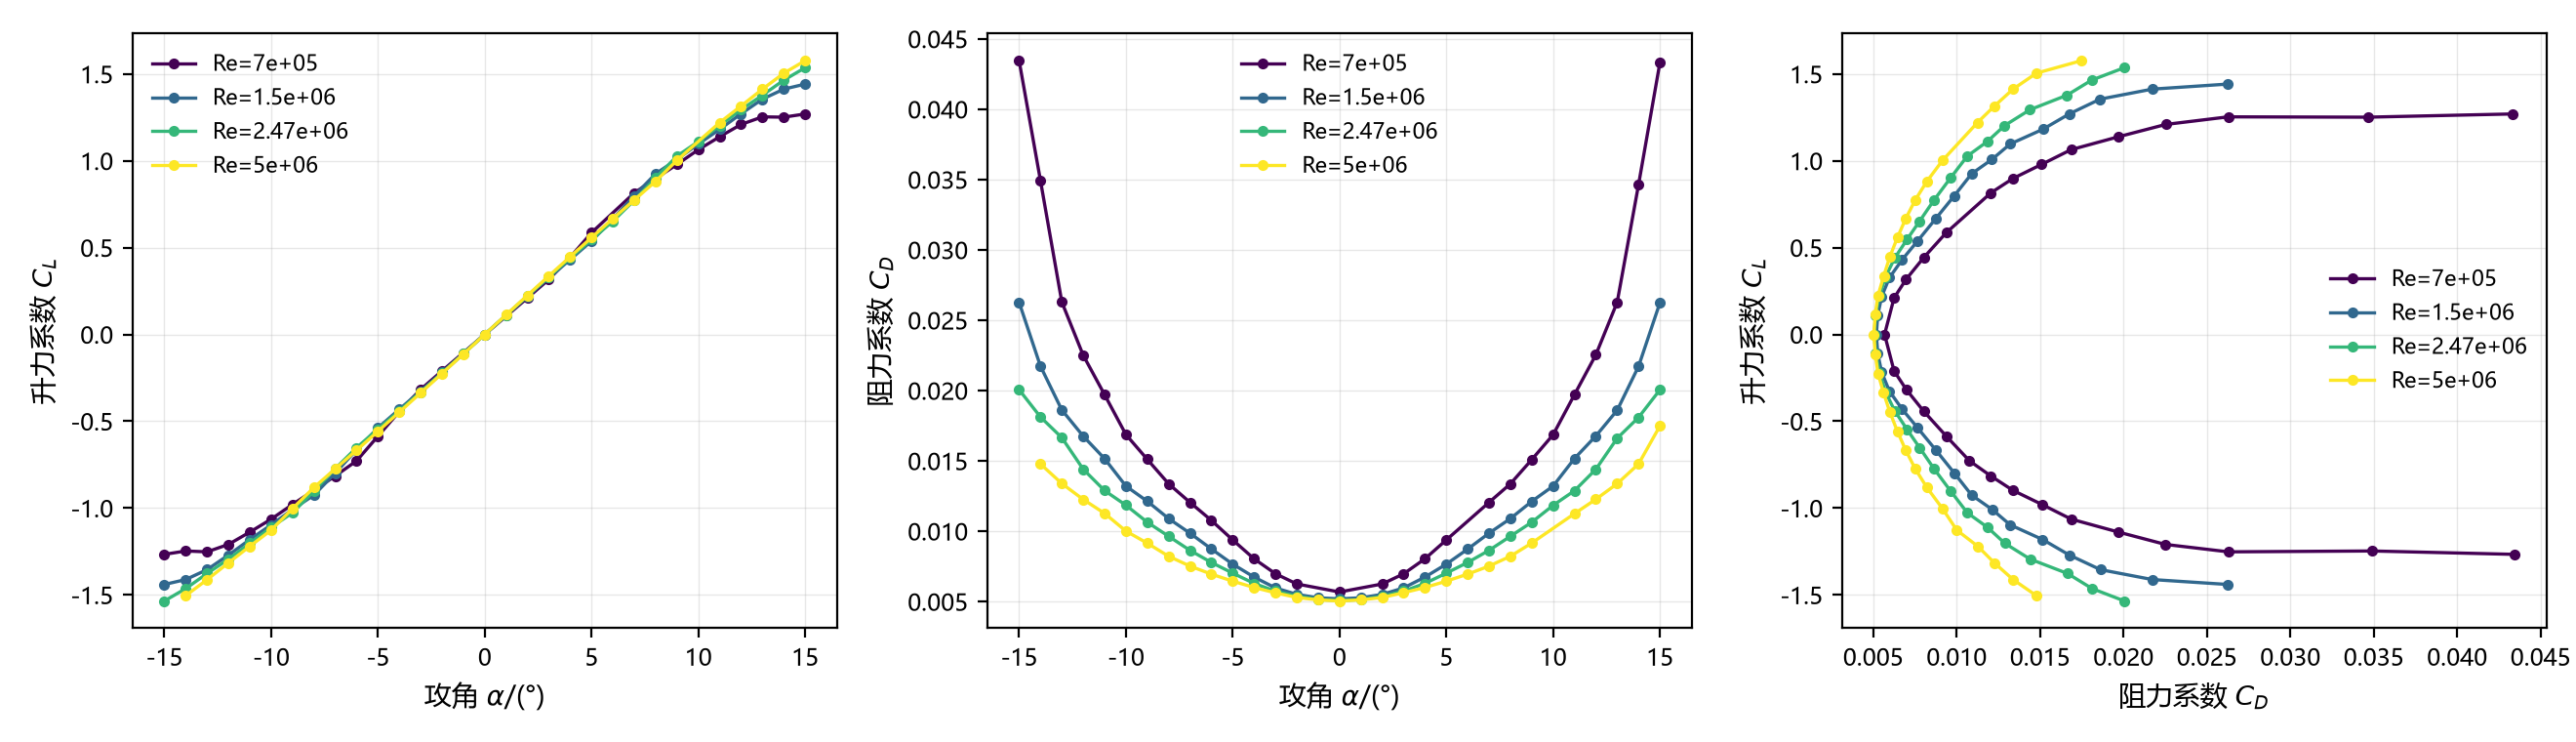
\includegraphics[width=0.94\textwidth]{figures/fig_1_2_polar.png}
\caption{翼帆翼型极线的 XFOIL 计算结果}
{\small Fig.~\thefigure\quad Airfoil polars of the wing sail computed by XFOIL\par}
\label{fig:polar}
\end{figure}
\FloatBarrier

\paragraph{全攻角范围扩展}
翼帆可绕桅旋转，其相对来流方向可覆盖一周，因此需要风帆在任意来流角下的气动数据。
XFOIL 仅在附着流区间内可靠收敛，本文采用"附着流段—过渡段—深失速段"三段拼接的方式，
将小攻角范围内的极线扩展至 $0^{\circ}\sim360^{\circ}$，使极线的攻角覆盖范围与由文件
导入的气动数据口径一致。记附着流可信攻角上限为 $\alpha_{\lim}$、过渡区宽度为 $w_b$，则

（1）当 $|\alpha|\le\alpha_{\lim}$ 时，按 $360^{\circ}$ 周期映射后取 XFOIL 结果：
\begin{equation}
\alpha_{\mathrm{eq}}=\left[\left(\alpha+180^{\circ}\right)\bmod 360^{\circ}\right]-180^{\circ},
\qquad C_{L,D}=C_{L,D}^{\mathrm{XFOIL}}\!\left(\alpha_{\mathrm{eq}}\right).
\label{eq:polar_xfoil}
\end{equation}

（2）当 $|\alpha|>\alpha_{\lim}+w_b$ 时，采用平板模型描述深失速段：
\begin{equation}
C_L=C_{D90}\sin\alpha\cos\alpha,
\qquad
C_D=C_{D90}\sin^2\alpha ,
\label{eq:flat_plate}
\end{equation}
式中 $C_{D90}$ 为平板在 $90^{\circ}$ 来流下的阻力系数。式\eqref{eq:flat_plate}~在
$0^{\circ}\sim360^{\circ}$ 内周期且对称，在 $90^{\circ}$、$270^{\circ}$ 处满足
$C_L=0$、$C_D=C_{D90}$，与平板正对来流的物理行为一致。

（3）当 $\alpha_{\lim}<|\alpha|\le\alpha_{\lim}+w_b$ 时，以余弦权重在 XFOIL 边界值与
平板模型之间平滑过渡：
\begin{equation}
w=\frac{1}{2}\left[1+\cos\!\left(\pi\frac{|\alpha|-\alpha_{\lim}}{w_b}\right)\right],
\qquad
C_{L,D}=w\,C_{L,D}^{\mathrm{XFOIL}}\!\Big|_{\pm\alpha_{\lim}}
+\left(1-w\right)C_{L,D}^{\mathrm{flat}} .
\label{eq:blend}
\end{equation}
权重 $w$ 由 1 连续降至 0，可保证极线在拼接点处的连续性，避免工作点寻优时出现虚假
局部极值。本文取 $\alpha_{\lim}=15^{\circ}$、$w_b=10^{\circ}$、$C_{D90}=1.8$，
全范围攻角步长为 $1^{\circ}$，拼接结果见图~\ref{fig:polar_full}。

\begin{figure}[htbp]
\centering
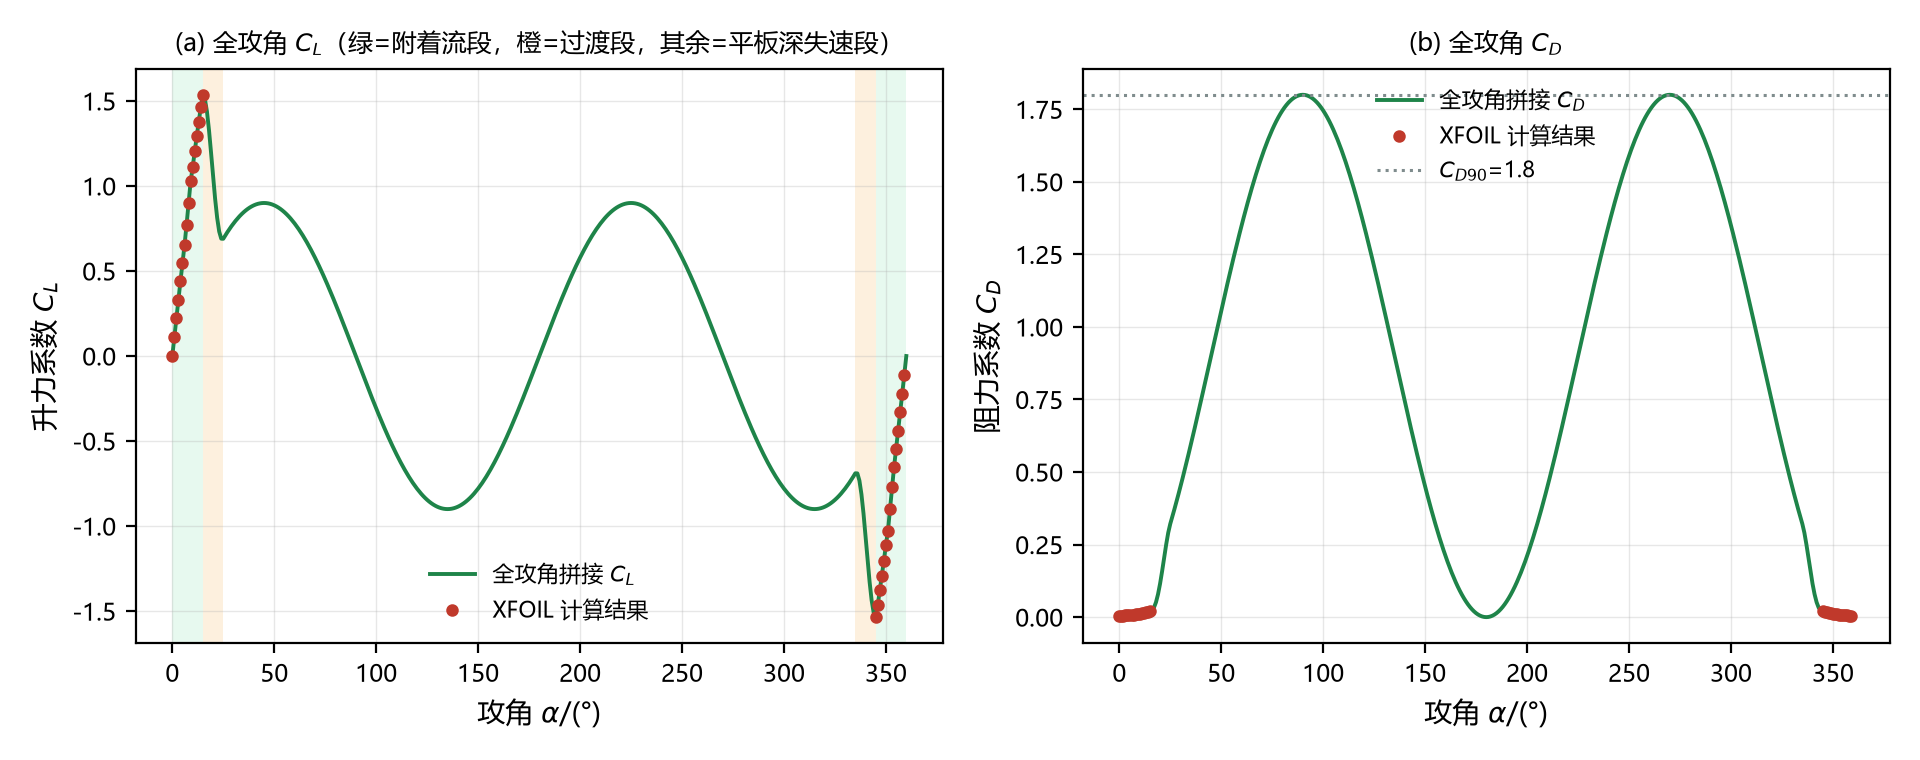
\includegraphics[width=0.90\textwidth]{figures/fig_1_2_polar_full.png}
\caption{全攻角极线的三段式拼接结果}
{\small Fig.~\thefigure\quad Three-segment extension of the polar over the full angle-of-attack range\par}
\label{fig:polar_full}
\end{figure}
\FloatBarrier

需要说明的是，式\eqref{eq:flat_plate}~与式\eqref{eq:blend}~构成的全攻角极线属工程
拼接结果，并非 CFD 或风洞实测数据，其大攻角段（$|\alpha|>25^{\circ}$）仅具量级意义，
用于表征风帆在任意来流角下的可用性能。此外，式\eqref{eq:polar_xfoil}~的周期映射
意味着同一组二维极线数据被用于全部来流方向，这在物理上要求帆能相对来流连续改变其
自身攻角，即要求转角可覆盖相应范围。

\subsubsection{转筒帆气动模型}
\label{sec:rotor_model}

转筒帆依靠马格努斯效应产生升力与推力，其气动特性由转筒比 $SR$、展弦比 $AR$ 与端板
直径比 $d_e/d$ 三个无量纲量决定：
\begin{equation}
SR=\frac{\Omega d}{2v},
\qquad
AR=\frac{H}{d},
\qquad
\frac{d_e}{d},
\label{eq:rotor_params}
\end{equation}
式中，$\Omega$ 为转筒角速度；$d$ 与 $H$ 分别为筒体直径与高度；$d_e$ 为端板直径。

本文采用文献\textsuperscript{\cite{demarco2016}}基于非定常 RANS 数值结果拟合的代理
模型计算转筒帆的升阻力系数。该模型考虑影响转子气动性能的关键参数，构建了多变量耦合
的多项式表达式，可量化转筒比、展弦比与端板直径比对气动系数的综合作用：
\begin{equation}
\begin{aligned}
C_L&=\sum_{i=1}^{4}\sum_{j=1}^{4}\sum_{k=1}^{3}a_{ijk}\,SR^{\,i}\,AR^{\,j}
\left(\frac{d_e}{d}\right)^{k},\\
C_D&=\sum_{i=1}^{4}\sum_{j=1}^{4}\sum_{k=1}^{3}b_{ijk}\,SR^{\,i}\,AR^{\,j}
\left(\frac{d_e}{d}\right)^{k},
\end{aligned}
\label{eq:rotor_surrogate}
\end{equation}
式中，$a_{ijk}$、$b_{ijk}$ 为经验系数，取自文献\textsuperscript{\cite{demarco2016}} 的
系数表（原文 Table~6），该表给出 $i=1\sim4$、$j=1\sim4$、$k=1\sim3$ 共 48 组系数，
本文程序所用系数与原文逐位一致。该模型的有效范围严格限定为 $1.0\le SR\le3.0$、
$2.0\le AR\le8.0$、$1.0\le d_e/d\le3.0$，覆盖了船舶应用中转筒帆的典型工况。

\begin{figure}[htbp]
\centering
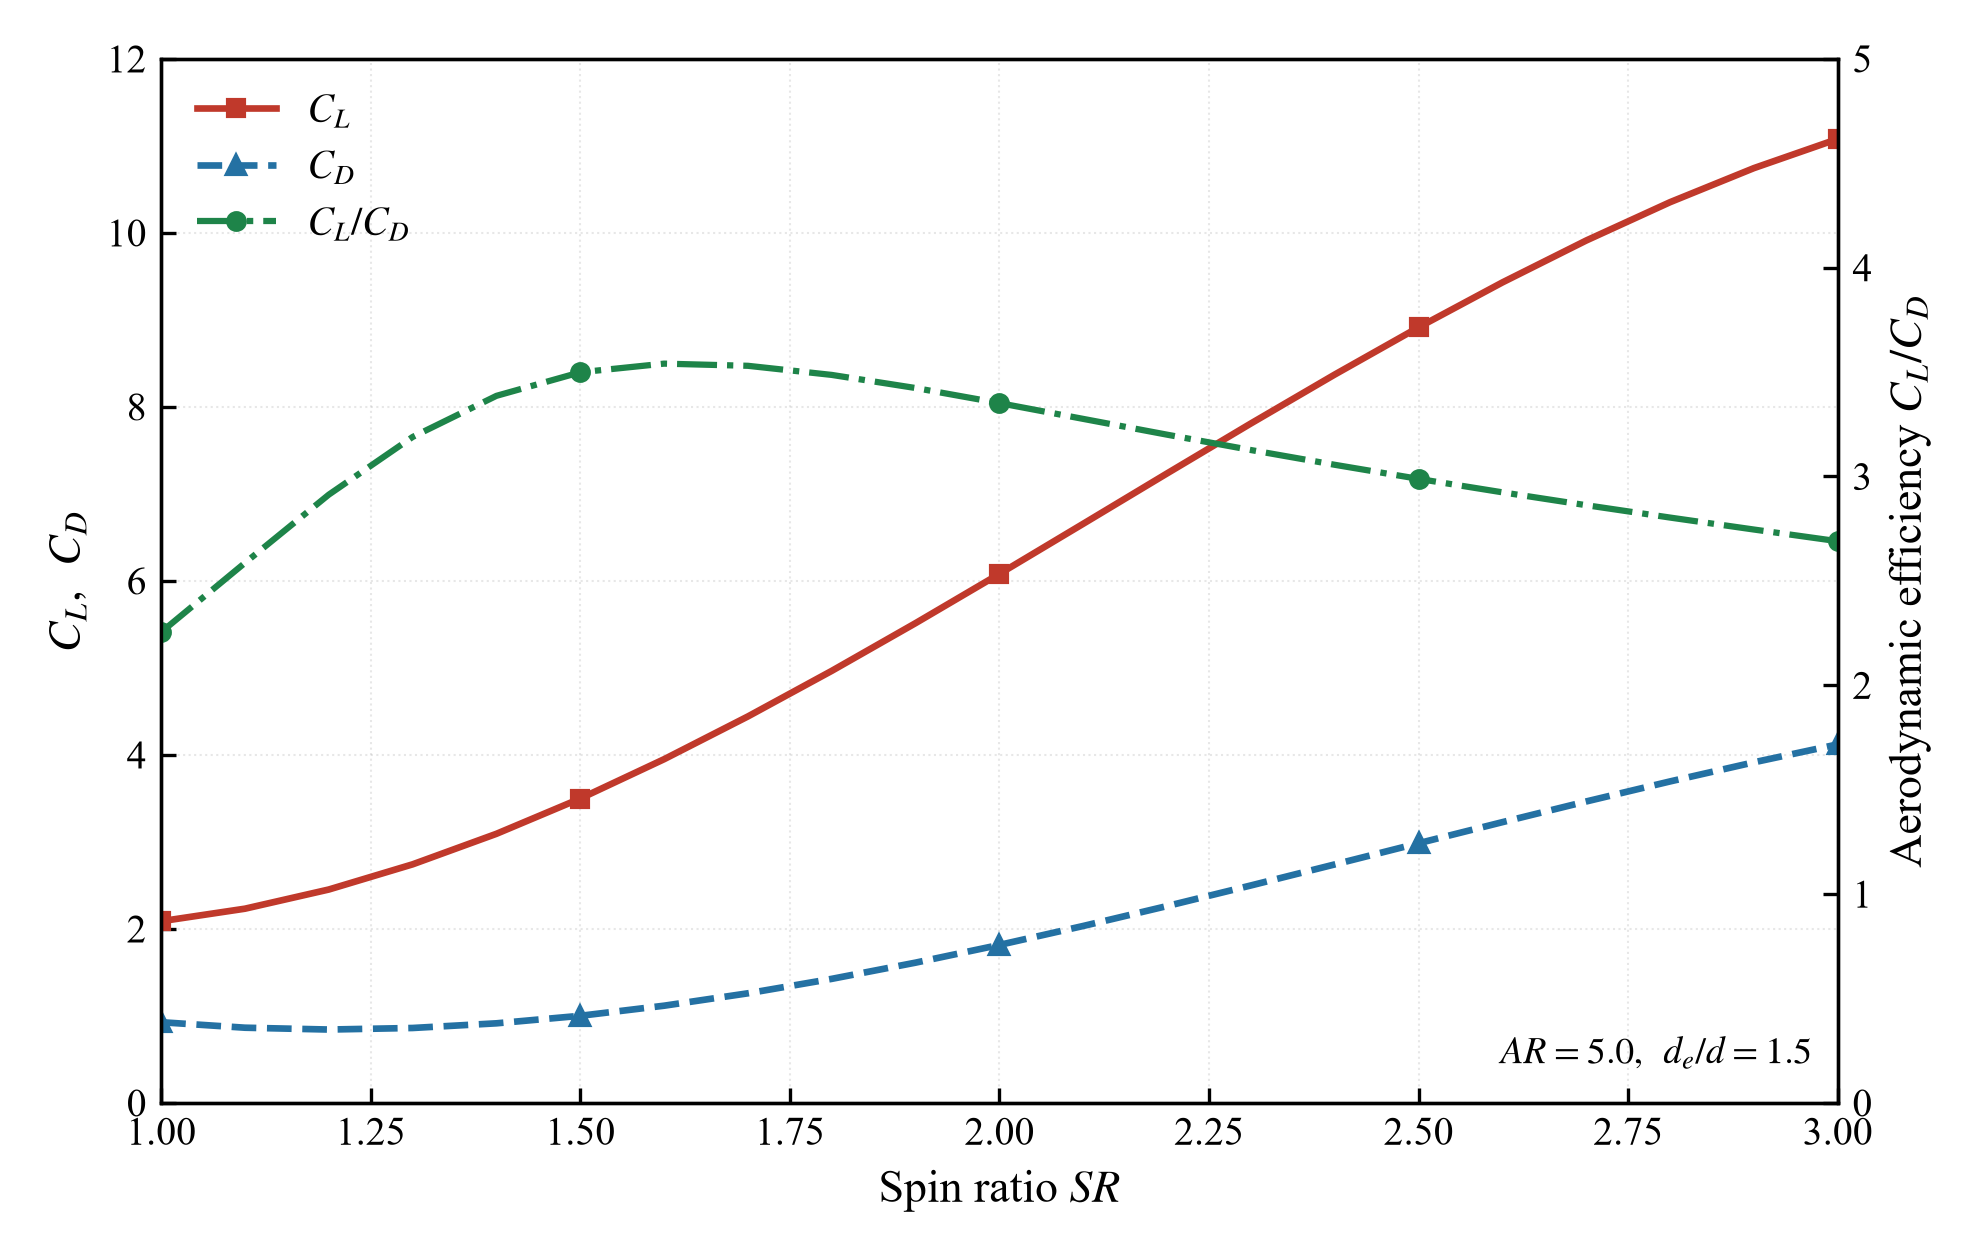
\includegraphics[width=0.78\textwidth]{figures/fig_1_2_rotor_polar.png}
\caption{转筒帆升阻力系数与气动效率随转筒比的变化（$AR=5.0$，$d_e/d=1.5$）}
{\small Fig.~\thefigure\quad Lift and drag coefficients and aerodynamic efficiency of the Flettner rotor against the spin ratio ($AR=5.0$, $d_e/d=1.5$)\par}
\label{fig:rotor_polar}
\end{figure}
\FloatBarrier

以程序界面默认的转筒几何 $d=3.0$~m、$H=15.0$~m、$d_e=4.5$~m（对应 $AR=5.0$、
$d_e/d=1.5$，参数均落在有效范围内）为例，取设计航速 12~kn，相对风速按
\S\ref{sec:wing_polar}~算例的 $3.83\sim16.17\ \mathrm{m\,s^{-1}}$ 范围变化，
$SR$ 在 $1.0\sim3.0$ 内取步长 0.5，得转筒帆的升阻力特性如表~\ref{tab:rotor_polar} 与
图~\ref{fig:rotor_polar} 所示。

\begin{table}[htbp]
\centering
\small
\setlength{\tabcolsep}{6pt}
\renewcommand{\arraystretch}{1.35}
\caption{转筒帆升阻力系数与最优工作点（$AR=5.0$，$d_e/d=1.5$，$d=3.0$~m）}
{\small Table~\thetable\quad Lift and drag coefficients and operating points of the Flettner rotor ($AR=5.0$, $d_e/d=1.5$, $d=3.0$~m)\par}
\smallskip
\label{tab:rotor_polar}
\begin{tabular}{@{}rrrrrr@{}}
\toprule
$SR$ & $C_L$ & $C_D$ & $C_L/C_D$ & $\Omega$/($\mathrm{rad\,s^{-1}}$) & $n$/($\mathrm{r\,min^{-1}}$) \\
\midrule
1.0 & 2.0865 & 0.9258 & 2.254 & 6.67 & 63.7 \\
1.5 & 3.4967 & 0.9995 & 3.498 & 10.00 & 95.5 \\
2.0 & 6.0790 & 1.8143 & 3.351 & 13.33 & 127.3 \\
2.5 & 8.9129 & 2.9831 & 2.988 & 16.67 & 159.2 \\
3.0 & 11.0780 & 4.1193 & 2.689 & 20.00 & 191.0 \\
\bottomrule
\end{tabular}
\end{table}
\FloatBarrier

表~\ref{tab:rotor_polar} 中转速以
$v=10\ \mathrm{m\,s^{-1}}$ 反算给出。可见转筒帆的升力系数随转筒比单调增大，
而气动效率 $C_L/C_D$ 在 $SR\approx1.6$ 处取最大值 3.54，此后随 $SR$ 增大而下降；
因此单纯提高转筒转速并不能持续提高助推效率，运行中需要按相对风速选择合适的工作点。
这与 1.2.4 节以助推力最大为目标的逐点寻优是一致的：寻优结果会自动落在效率与
$C_L$ 的综合最优点上。

\subsubsection{助推力合成与工作点选取}
\label{sec:sail_operating_point}

\paragraph{升阻力到助推力与侧推力}
设风帆投影面积为 $A$、数量为 $N$，相对风动压为 $\tfrac{1}{2}\rho v^2$，则风帆产生的
升力与阻力为
\begin{equation}
F_L=\frac{1}{2}\rho v^2ANC_L,
\qquad
F_D=\frac{1}{2}\rho v^2ANC_D .
\label{eq:lift_drag}
\end{equation}
翼帆取 $A$ 为单面受风面积、$N=N_s$；转筒帆取 $A=dH$、$N=N_r$。式\eqref{eq:lift_drag}~
中的动压必须按相对风速 $v$ 计算。若误用船速，则助推力将仅随航速变化而丧失对真实风场
的响应，顺风增益、顶风减益的物理规律将不再成立。

将升阻力在船舶航向与垂直航向方向合成，得助推力 $F_T$、侧推力 $F_S$ 及相应的推力系数
$C_X$、侧推力系数 $C_Y$（图~\ref{fig:sail_force} 中对应的无量纲力分别为 $F_X$、$F_Y$）：
\begin{equation}
\begin{aligned}
F_T&=\frac{1}{2}\rho v^2AC_L\sin\beta-\frac{1}{2}\rho v^2AC_D\cos\beta,\\
F_S&=\frac{1}{2}\rho v^2AC_L\cos\beta+\frac{1}{2}\rho v^2AC_D\sin\beta,
\end{aligned}
\label{eq:thrust_decomp}
\end{equation}
\begin{equation}
\begin{aligned}
C_X&=C_L\sin\beta-C_D\cos\beta,\\
C_Y&=C_L\cos\beta+C_D\sin\beta .
\end{aligned}
\label{eq:force_coef}
\end{equation}
式\eqref{eq:thrust_decomp}、\eqref{eq:force_coef}~中的面积与数量因子在写成推力系数
形式时略去。当风向角与风翼几何确定后，改变攻角 $\alpha$ 即可得到推力系数 $C_X$、
侧推力系数 $C_Y$ 与 $\alpha$ 的关系曲线 $C_X$--$\alpha$、$C_Y$--$\alpha$，以及风翼
升阻极坐标曲线 $C_L$--$C_D$；结合式\eqref{eq:coef_functions}~有
\begin{equation}
\begin{aligned}
C_X&=f\!\left(\alpha,\lambda,\varepsilon\right)\sin\beta
     -g\!\left(\alpha,\lambda,\varepsilon\right)\cos\beta,\\
C_Y&=f\!\left(\alpha,\lambda,\varepsilon\right)\cos\beta
     +g\!\left(\alpha,\lambda,\varepsilon\right)\sin\beta .
\end{aligned}
\label{eq:force_coef_alpha}
\end{equation}


\paragraph{最优工作点选取}
对第 $i$ 个航路点，以助推力最大为目标确定风帆工作点。翼帆以攻角为搜索变量：
\begin{equation}
\alpha_i^{*}=\arg\max_{\alpha_j}
\left[F_L\!\left(\alpha_j\right)\sin\beta_i-F_D\!\left(\alpha_j\right)\cos\beta_i\right],
\qquad
F_{T,i}=\max\!\left(0,\ \max_j\left[\cdot\right]\right);
\label{eq:opt_alpha}
\end{equation}
转筒帆以转筒比为搜索变量：
\begin{equation}
SR_i^{*}=\arg\max_{SR_j}
\left[F_L\!\left(SR_j\right)\sin\beta_i-F_D\!\left(SR_j\right)\cos\beta_i\right],
\qquad
F_{T,i}=\max\!\left(0,\ \max_j\left[\cdot\right]\right).
\label{eq:opt_sr}
\end{equation}
式\eqref{eq:opt_alpha}、\eqref{eq:opt_sr}~在完整气动数据表上逐点遍历求解，各航路点
相互独立；当所有候选工作点均产生负推力时取 $F_{T,i}=0$，对应收帆或停转状态。
由于寻优为穷举，最优解的精度直接由数据表步长决定。

\subsubsection{小结}

本节建立了翼帆与转筒帆的统一气动计算模型与计算流程。在统一的坐标与角度体系下，
翼帆气动特性由 XFOIL 计算的二维极线表征，并经三段拼接扩展至全攻角范围；转筒帆气动
特性由基于非定常 RANS 数值结果拟合的多项式代理模型给出；两者以统一的升阻力合成关系
折算至船舶航向与垂直航向，并逐航路点以助推力最大为目标确定工作点。本节输出的
逐航路点助推力构成后续船机桨帆匹配及航程节油计算的输入。
\subsection{船舶阻力与螺旋桨工作点计算}
\label{sec:ship_propeller}
翼帆提供的纵向推力能够降低船舶对螺旋桨推力的需求，同时改变螺旋桨工作点及推进效率。因此，本文结合船舶静水阻力、船体与螺旋桨相互作用参数及螺旋桨敞水特性，分别计算无帆和翼帆助推工况下的推进功率，为后续燃油消耗评估提供依据。本文以单桨船定航速准稳态航行为对象，计算过程中保持船舶航速及螺旋桨几何参数不变，并假定伴流分数、推力减额系数和相对旋转效率不随翼帆助推载荷变化。

\subsubsection{船舶静水阻力计算}

船舶静水阻力可通过导入阻力数据并按航速插值得到，也可采用程序集成的 Holtrop--Mennen 经验方法计算。经验方法将总阻力表示为
\begin{equation}
R_T=(1+k_1)R_F+R_{\mathrm{APP}}+R_W+R_B+R_{\mathrm{TR}}+R_A.
\label{eq:resistance}
\end{equation}
式中，$R_F$ 为船体摩擦阻力，$1+k_1$ 为船体形状因子，$R_{\mathrm{APP}}$ 为附体阻力，$R_W$ 为兴波阻力，$R_B$ 为球鼻首附加阻力，$R_{\mathrm{TR}}$ 为浸没艉板附加阻力，$R_A$ 为模型与实船相关修正阻力。其中，摩擦阻力按照下式计算：
\begin{equation}
\begin{aligned}
R_F&=\frac{1}{2}\rho_w V_s^2 S C_F,\\
C_F&=\frac{0.075}{(\log_{10}Re-2)^2},\qquad Re=\frac{V_sL_{pp}}{\nu}.
\end{aligned}
\label{eq:friction}
\end{equation}
式中，$\rho_w$ 为水密度，$V_s$ 为船舶航速，$S$ 为船体湿表面积，$L_{pp}$ 为垂线间长，$\nu$ 为水的运动黏度。

程序依据船舶主尺度、方形系数、中横剖面系数及浮心纵向位置等参数，在给定航速范围内建立阻力曲线。当前经验公式计算采用正浮及常规艉型假设，并将球鼻首面积、浸没艉板面积和附体面积设为零，因此相应阻力项不计入计算。Holtrop-Mennen 方法适用于长度在 50 至 500 米之间的船只。不建议将其应用于小型船只（排水量小于 30 米）。在小型船只上，雷诺数依赖性和回归系数并不稳定。对于上述的船舶，应补充相应参数或采用能够反映实际船型的阻力数据。

\subsubsection{船体与螺旋桨相互作用}

采用伴流分数 $w$、推力减额系数 $t$ 和相对旋转效率 $\eta_R$ 描述船体与螺旋桨的相互作用。在经验公式模式下，单桨船伴流分数采用基于 Harvald 数据的经验拟合关系\textsuperscript{\cite{harvald1983,molland2011}}，推力减额系数采用与伴流分数相关的近似关系\textsuperscript{\cite{molland2011}}：
\begin{equation}
\begin{aligned}
w&=1.095-3.4C_B+3.3C_B^2
+\frac{0.5C_B^2(6.5-L_{pp}/B)}{L_{pp}/B},\\
t&=k_Rw.
\end{aligned}
\label{eq:wake}
\end{equation}
式中，$C_B$ 为方形系数，$B$ 为船宽，$k_R$ 为舵型修正系数。计算中，$w$ 和 $t$ 对同一船型取定值，$\eta_R$ 由输入参数给定，缺少相关数据时取默认值 1.0。采用外部数据时，则按航速对上述参数进行插值。

对于第 $i$ 个航路点，设翼帆纵向助推力为 $F_{T,i}$，则螺旋桨所需推力及其进速分别为
\begin{equation}
T_{P,i}=\frac{R_T(V_s)-F_{T,i}}{1-t},\qquad V_a=(1-w)V_s.
\label{eq:required_thrust}
\end{equation}
无帆工况取 $F_{T,i}=0$。其中，$R_T-F_{T,i}$ 表示需要由螺旋桨承担的剩余纵向力需求。本文暂不计入翼帆侧向力引起的漂角、横倾及操舵附加阻力。

\subsubsection{螺旋桨敞水特性与工作点求解}
\label{sec:propeller-open-water}

为适应不同的输入条件，本文提供敞水特性数据导入、已知几何参数的性能计算以及基于图谱回归的设计点匹配三种方式，获得螺旋桨敞水特性。各方式统一采用进速系数 $J$、推力系数 $K_T$、转矩系数 $K_Q$ 和敞水效率 $\eta_0$ 描述螺旋桨性能，其定义为
\begin{equation}
\begin{aligned}
J&=\frac{V_a}{nD},& K_T&=\frac{T_P}{\rho_w n^2D^4},\\
K_Q&=\frac{Q}{\rho_w n^2D^5},& \eta_0&=\frac{JK_T}{2\pi K_Q}.
\end{aligned}
\label{eq:open_water}
\end{equation}
式中，$V_a$ 为螺旋桨进速，$n$ 为转速，单位为 $\mathrm{s}^{-1}$；$D$ 为螺旋桨直径，$T_P$ 为推力，$Q$ 为敞水转矩，$\rho_w$ 为水密度。

对于已有敞水性能数据的螺旋桨，采用\textbf{数据导入方式}，读取不同进速系数下的推力系数、转矩系数及敞水效率，并结合给定的螺旋桨直径建立包含上述4个性能数据的数据集。

对于几何参数已知但缺少敞水性能数据的螺旋桨，采用\textbf{已知几何参数的性能计算方式}。输入螺旋桨直径 $D$、螺距比 $P/D$、叶数 $Z$ 和盘面比 $A_E/A_0$，选择相应的系列桨回归关系，在给定进速系数范围内逐点计算 $K_T$ 和 $K_Q$，并由式\eqref{eq:open_water}求得敞水效率，形成完整的敞水特性曲线。计算过程中保持输入几何参数不变，不进行螺距比迭代。程序支持 Wageningen B 系列及 KA+19A 导管桨，并按所选系列调用对应的回归计算关系。

对于需要根据船舶设计工况确定螺旋桨参数的情况，采用\textbf{基于图谱回归的设计点匹配方式}。首先根据设计航速 $V_{s,d}$ 下的船舶阻力 $R_{T,d}$、伴流分数 $w$ 和推力减额系数 $t$，确定设计推力 $T_{P,d}=R_{T,d}/(1-t)$ 与进速 $V_{a,d}=(1-w)V_{s,d}$。在给定设计转速 $n_d$ 后，当前程序取螺旋桨直径 $D=0.675T_s$，其中 $T_s$ 为船舶吃水，并将盘面比固定为 0.75。根据式\eqref{eq:open_water}计算设计进速系数及目标推力系数，随后迭代调整螺距比，使图谱回归得到的推力系数与设计工况下，满足船舶推进需求所需的推力系数匹配。完成匹配后，固定所得几何参数，计算不同进速系数下的敞水特性曲线。该方式以满足设计点推力需求为目标，未进行螺旋桨直径与推进效率的联合优化。上述两种计算方式均以系列桨图谱回归为基础，其区别在于前者直接计算已知几何参数的性能，后者通过迭代确定满足设计工况的螺距比。

以三种方式获得的敞水数据都可进入后续统一的求解流程。对于第 $i$ 个航路点，根据船舶阻力及翼帆纵向推力确定螺旋桨所需推力 $T_{P,i}$。由式\eqref{eq:open_water}消去转速，可得
\begin{equation}
\frac{K_T(J_i)}{J_i^2}=\frac{T_{P,i}}{\rho_w V_a^2D^2}.
\label{eq:operating_point}
\end{equation}
三种方式获得的敞水特性曲线描述了螺旋桨在不同工况下的性能。为计算翼帆助推后的推进功率，需根据各航路点的推力需求确定相应的螺旋桨工作点。本文在航速及螺旋桨几何参数保持不变的条件下，由式\eqref{eq:operating_point}计算推力匹配参数，并通过敞水曲线插值得到对应的进速系数和敞水效率。分别对无帆与有帆工况进行上述计算，以考虑翼帆助推引起的螺旋桨负荷及效率变化。

\subsubsection{助推工况下的推进功率}

根据船体效率和螺旋桨敞水效率，推进效率表示为
\begin{equation}
\eta_{D,i}=\eta_{0,i}\eta_R\eta_H,\qquad \eta_H=\frac{1-t}{1-w}.
\label{eq:efficiency}
\end{equation}
由此得到翼帆助推工况下的螺旋桨收到功率：
\begin{equation}
P_{D,i}=\frac{\left[R_T(V_s)-F_{T,i}\right]V_s}{\eta_{D,i}}.
\label{eq:power}
\end{equation}
无帆工况采用相同方法，以 $F_{T,i}=0$ 重新求解工作点及推进功率。上述方法同时考虑了翼帆推力对推进负荷的直接削减，以及工作点变化引起的敞水效率变化，可为后续结合主机负荷与燃油消耗率的节油计算提供功率输入。计算适用于剩余推力需求为正、工作点处于有效敞水数据范围内的工况，且未显式计入轴系传动损失。

\subsection{主机燃油消耗与航程节油率计算}
\todo{根据推进功率和负荷相关燃油消耗率计算航段油耗，积分或累加得到航程总油耗，并定义节油量与节油率。}

\section{计算流程与模型验证}
\subsection{计算流程及程序实现}
本程序总计算流程如图~\ref{fig:calculation-flow} 所示。

\begin{figure}[htbp]
\centering
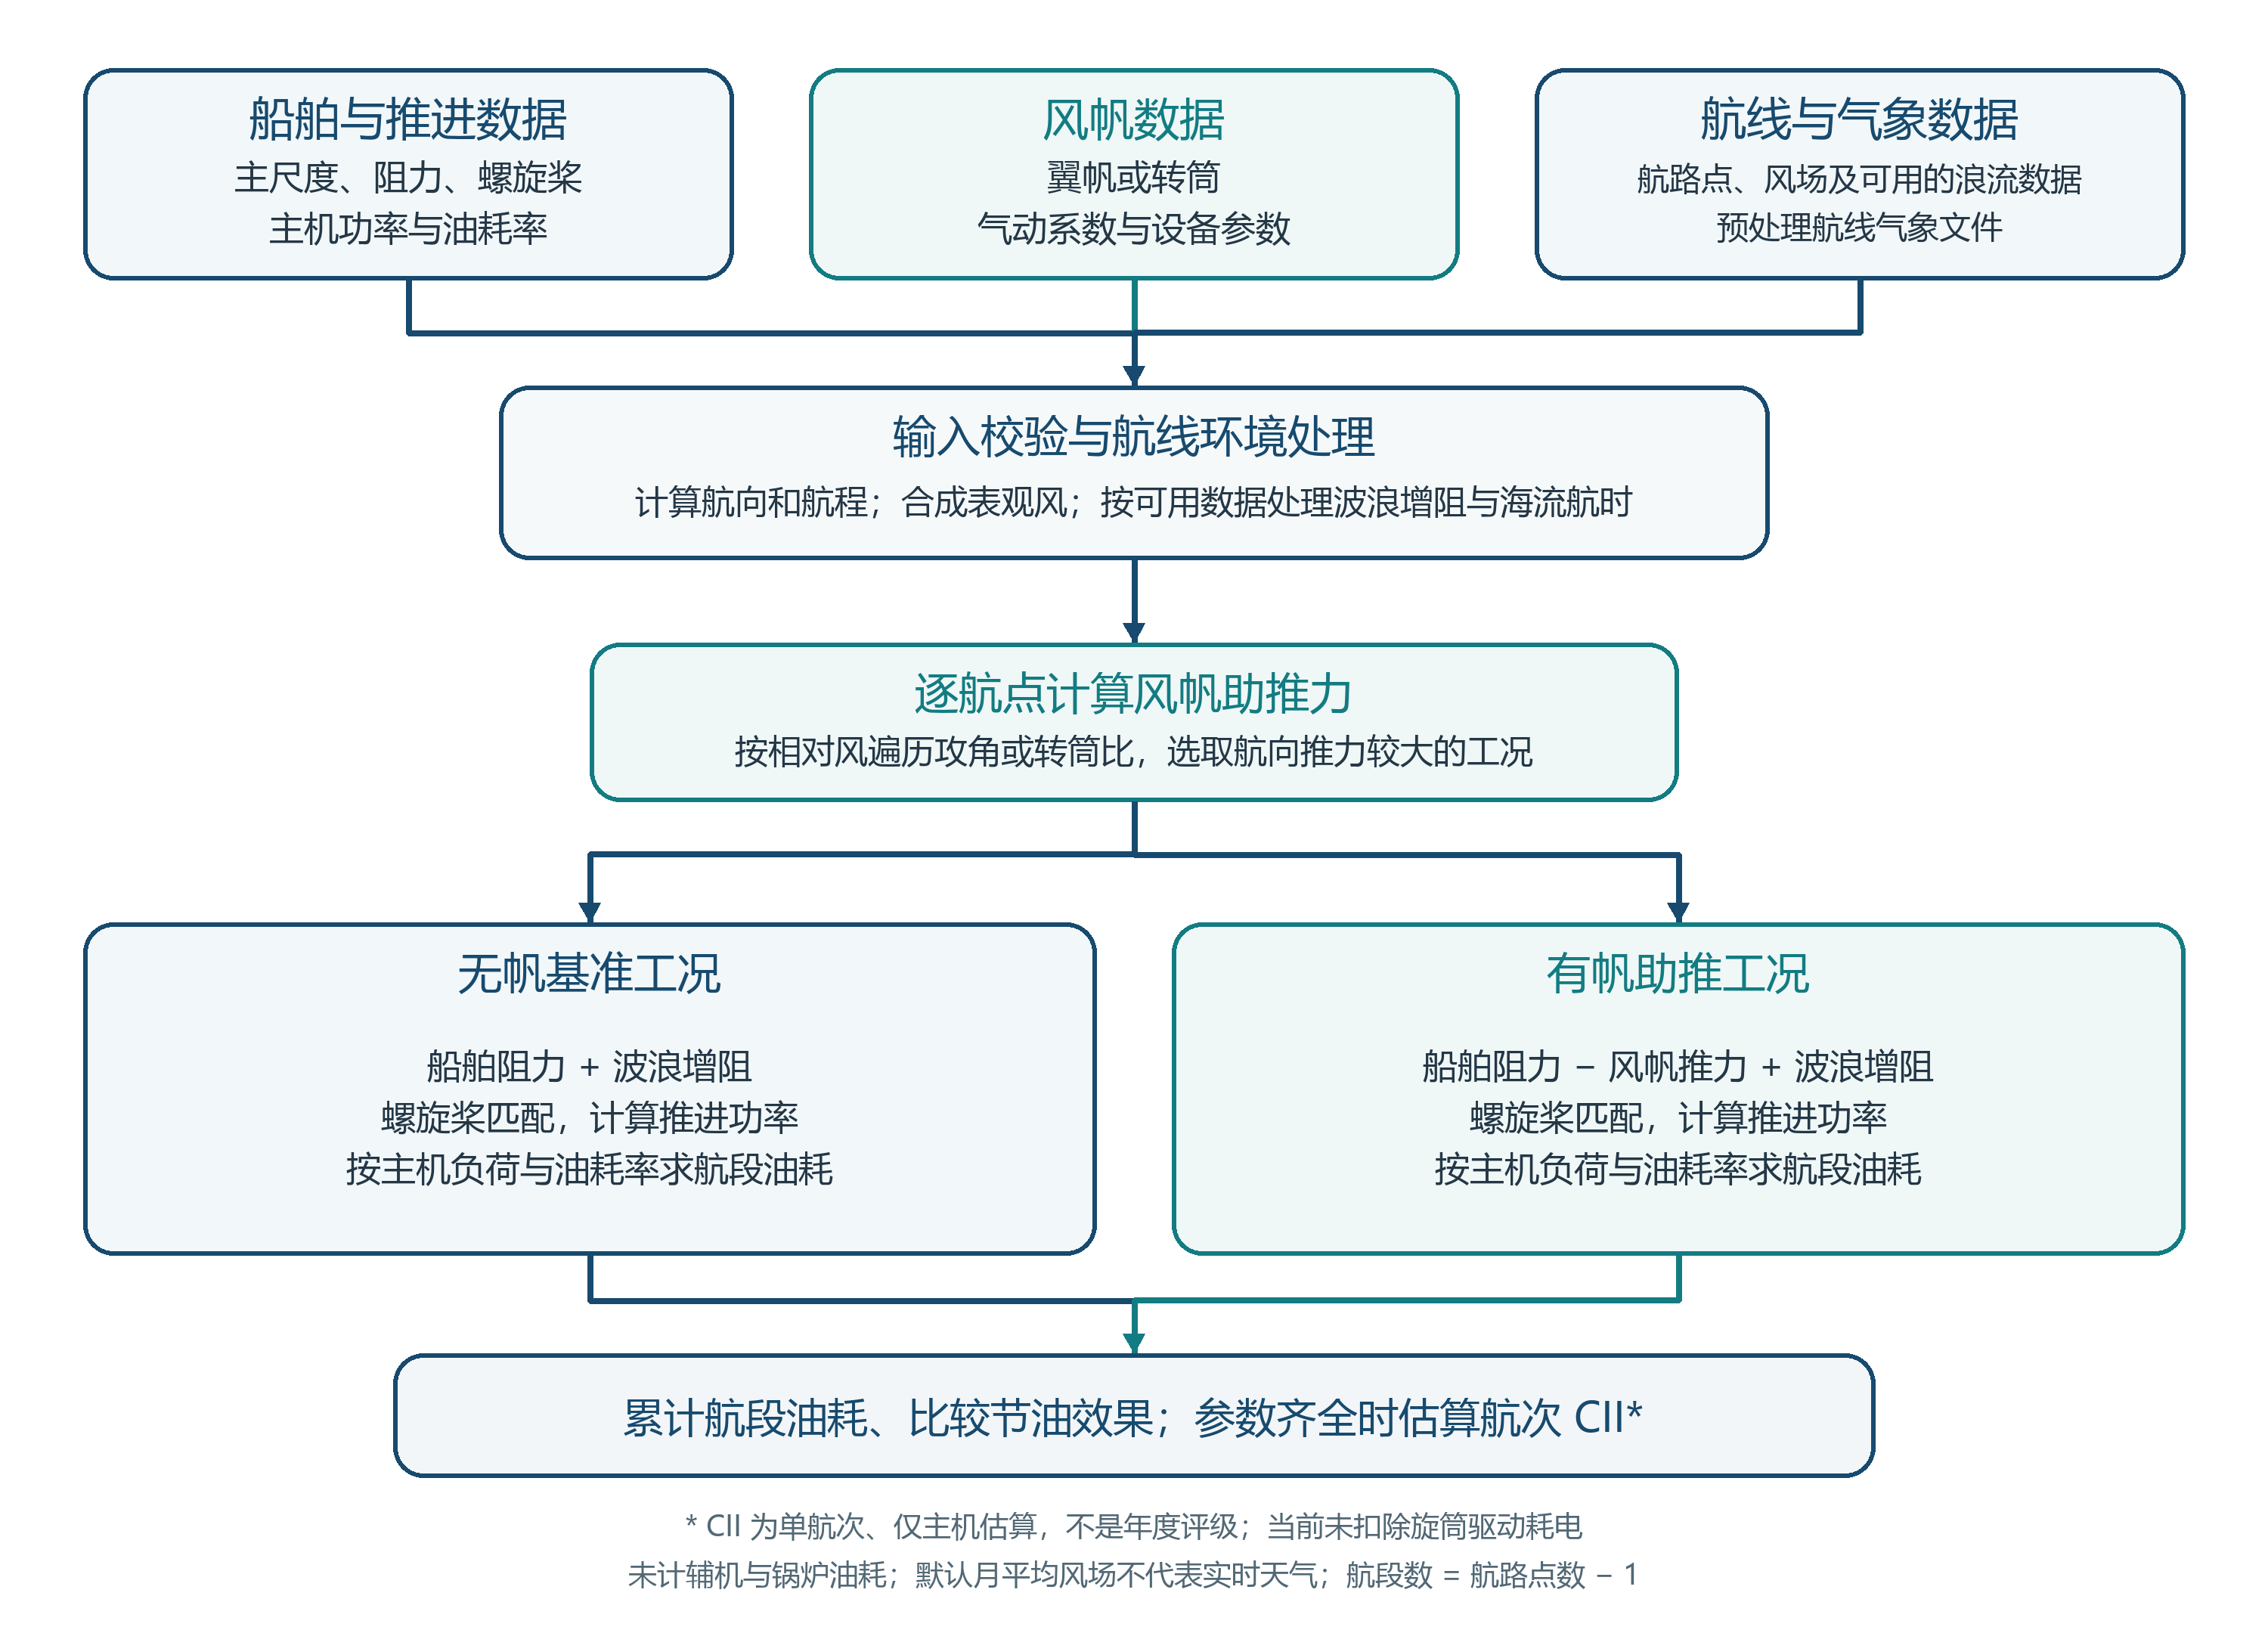
\includegraphics[width=0.85\linewidth]{figures/calculation-flow.png}
\caption{风帆助推船舶航次能耗计算流程}
\label{fig:calculation-flow}
\end{figure}


本文建立的计算程序用于估算船舶在给定航线和航速下，安装风帆助推装置前后的推进功率与主机燃油消耗，并据此比较航次层面的节油效果。程序由船舶参数、风帆助推、航线气象和结果分析等模块组成。计算以航线相邻航路点构成的航段为基本单元，依次完成环境数据处理、助推力计算、船舶推进功率计算和燃油消耗积分。

计算开始前，程序读取用户设置的船舶航速、船舶主参数、航线以及船舶阻力、螺旋桨和主机油耗率数据。船舶阻力数据可由 Excel 导入，也可由程序内的阻力计算模块生成。两种方式统一整理为航速、阻力、伴流分数、推力减额分数和相对旋转效率五列。程序检查阻力数据的列数、数值有效性及航速递增关系，并要求计算航速处于阻力数据覆盖范围内。螺旋桨静水特性有3种导入方式：对于已有敞水性能数据的螺旋桨，采用Excel数据导入方式；对于几何参数已知但缺少敞水性能数据的螺旋桨，采用已知几何参数的性能计算方式；对于需要根据船舶设计工况确定螺旋桨参数的情况，采用基于图谱回归的设计点匹配方式。这三种方式的具体计算细节在\ref{sec:propeller-open-water}中有详细阐释。主机油耗率用Excel导入即可。各数据导入界面见图~\ref{fig:ui-ship-inputs}。

\begin{figure}[htbp]
\centering
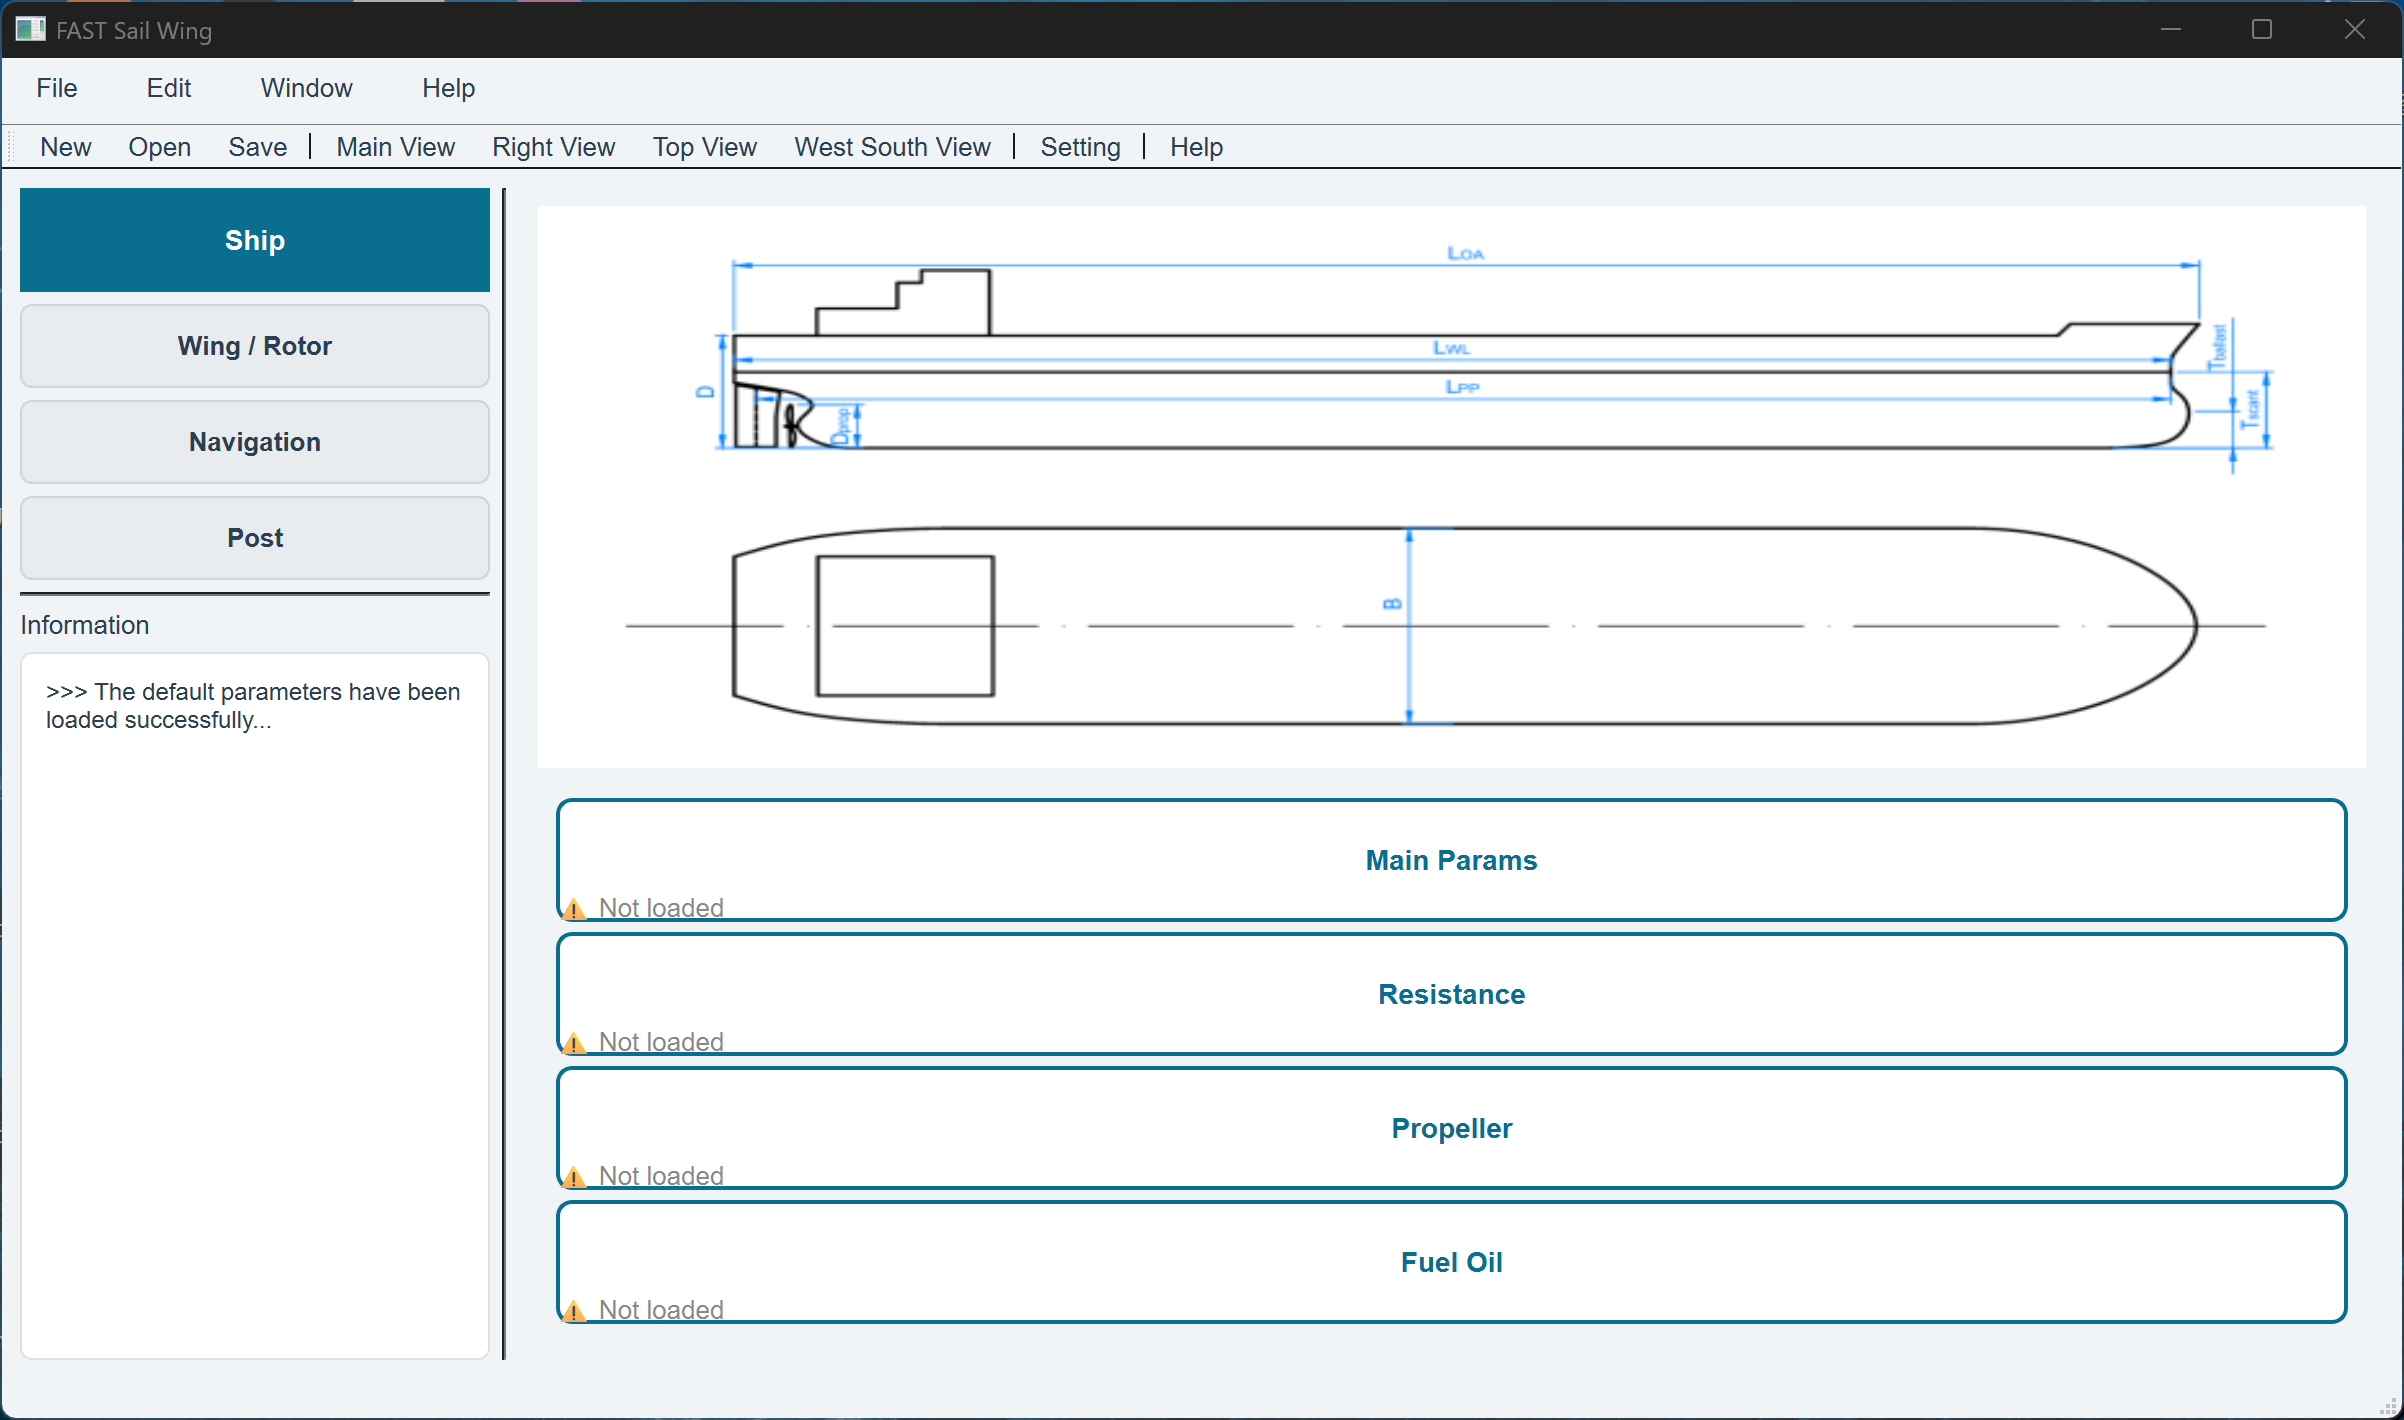
\includegraphics[width=0.95\linewidth]{figures/ui-ship.png}
\caption{船舶参数模块界面}
\label{fig:ui-ship}
\end{figure}


\begin{figure}[htbp]
\centering
\begin{minipage}{0.48\linewidth}
\centering
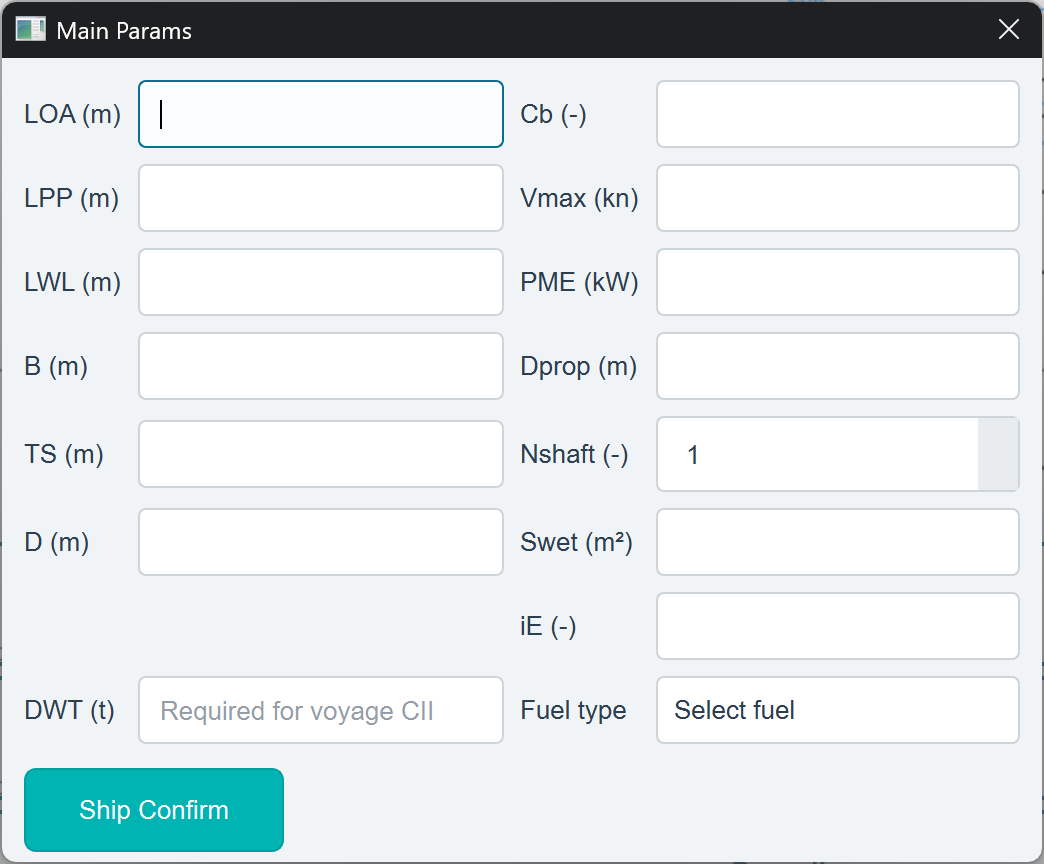
\includegraphics[width=\linewidth]{figures/ui-particulars.png}
\par\small （a）船舶主尺度
\end{minipage}\hfill
\begin{minipage}{0.48\linewidth}
\centering
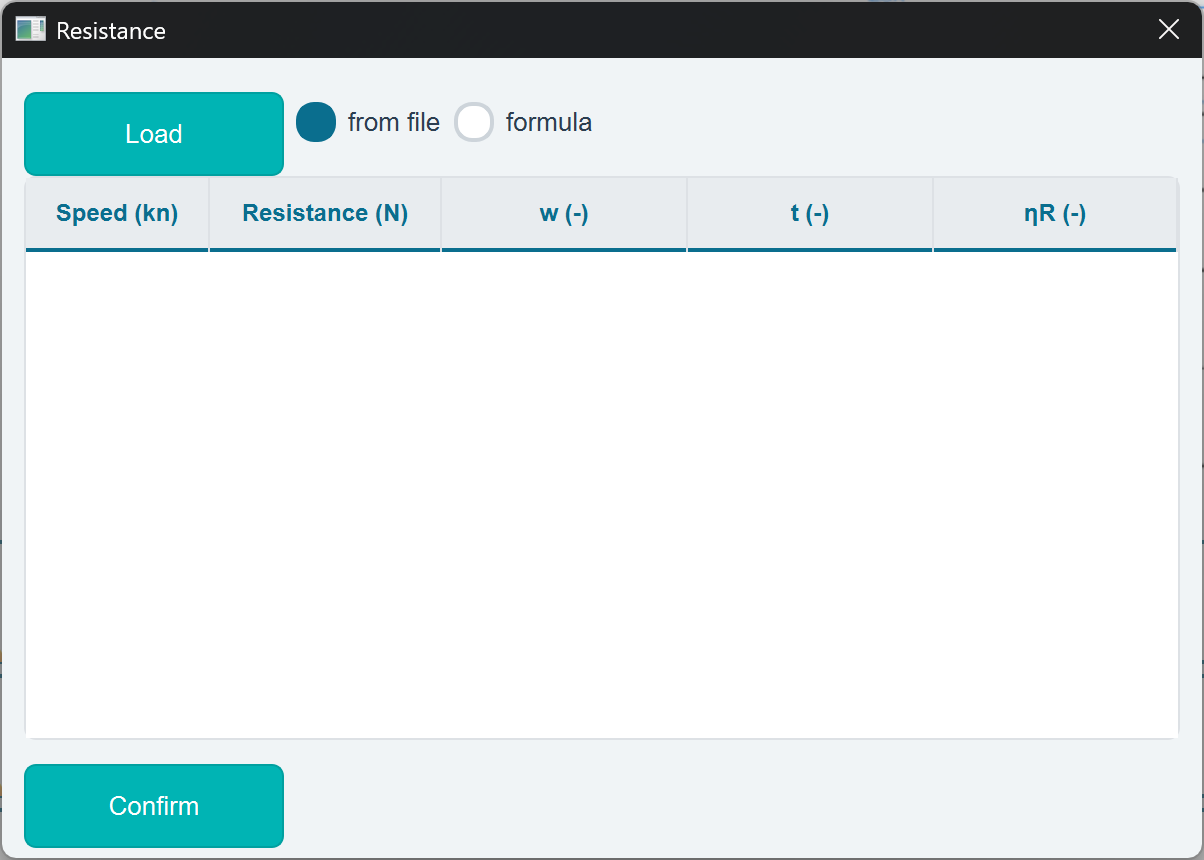
\includegraphics[width=\linewidth]{figures/ui-resistance.png}
\par\small （b）阻力
\end{minipage}
\par\medskip
\begin{minipage}{0.48\linewidth}
\centering
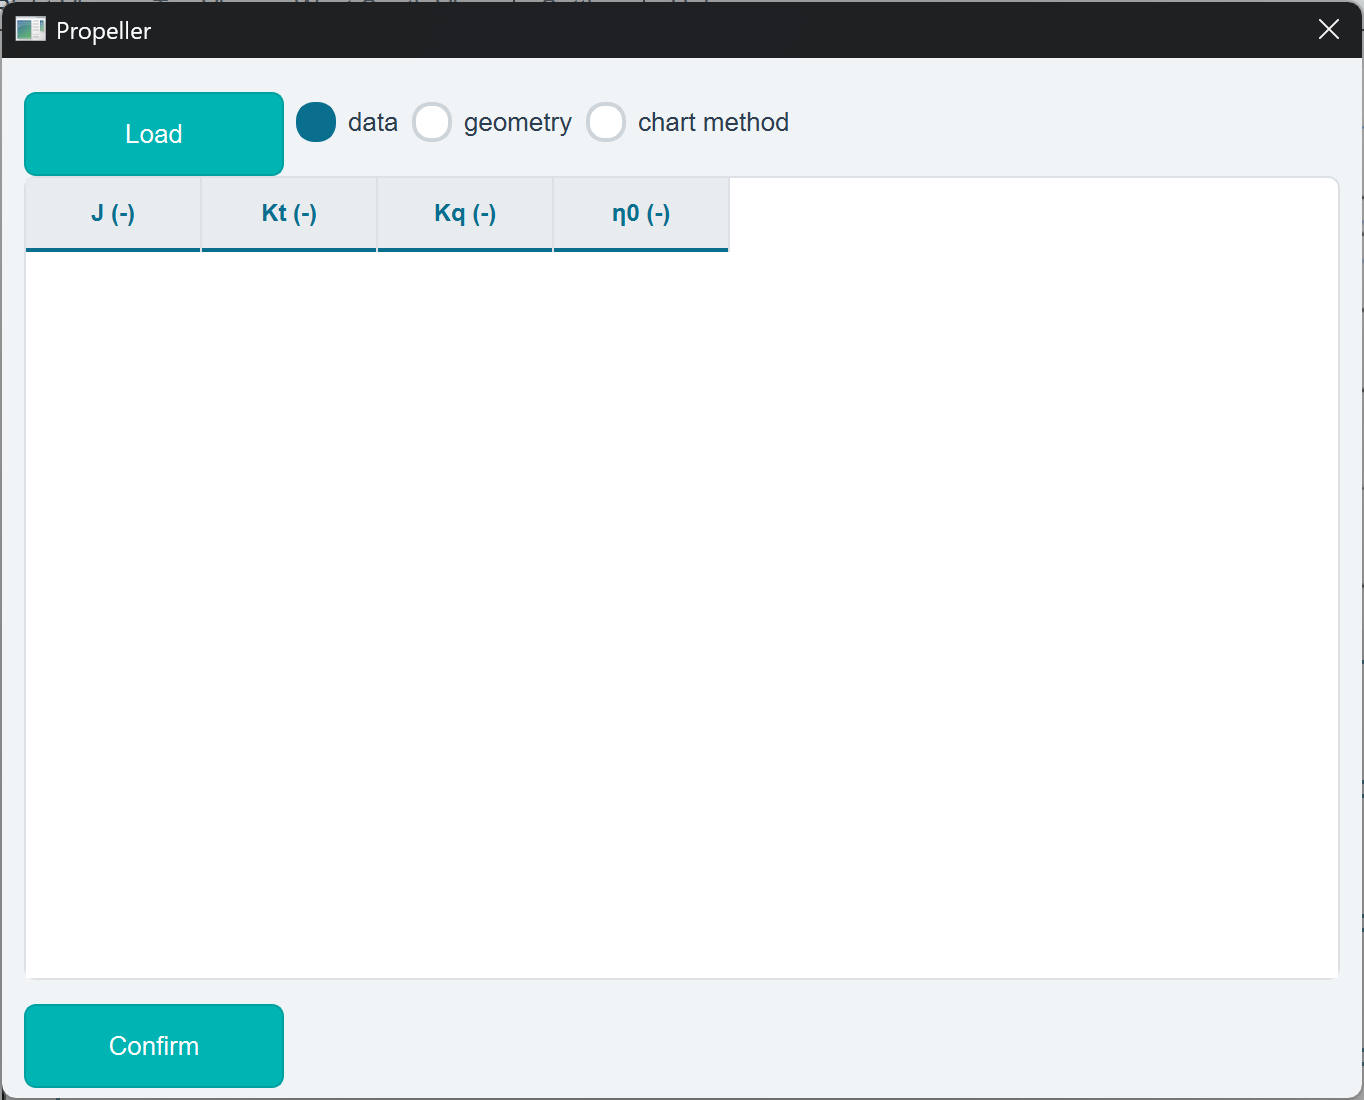
\includegraphics[width=\linewidth]{figures/ui-propeller.png}
\par\small （c）螺旋桨静水特性
\end{minipage}\hfill
\begin{minipage}{0.48\linewidth}
\centering
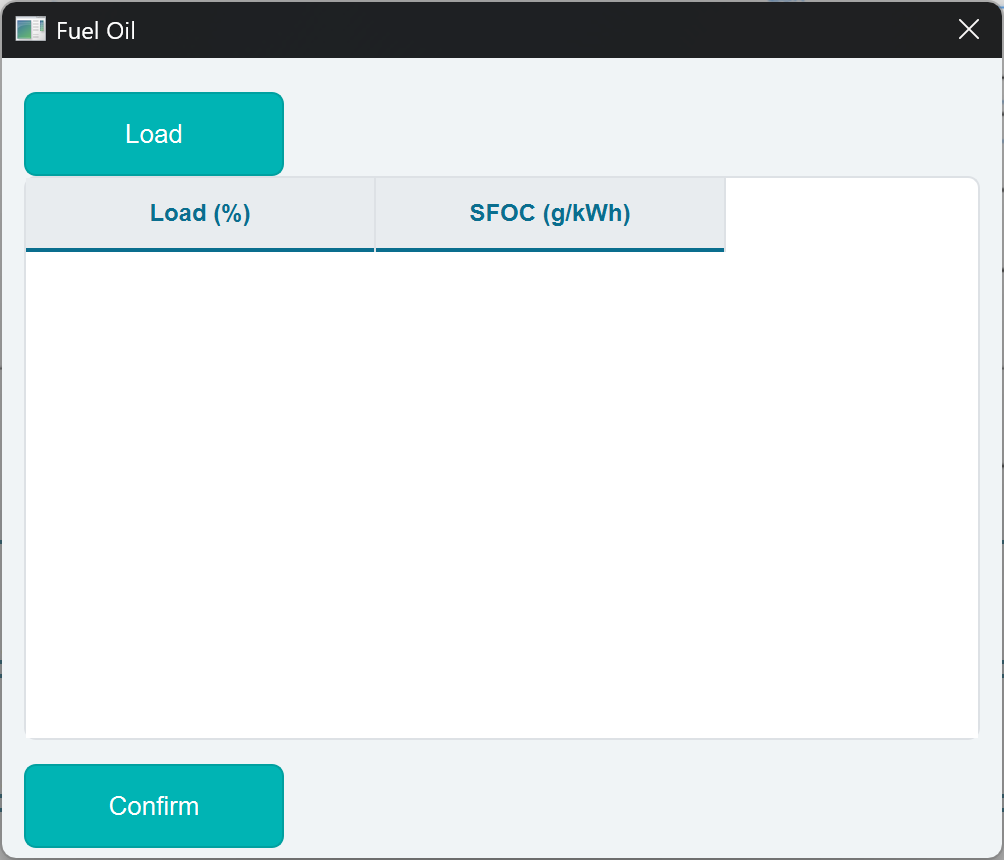
\includegraphics[width=\linewidth]{figures/ui-sfoc.png}
\par\small （d）主机油耗
\end{minipage}
\caption{船舶参数与推进性能数据输入界面}
\label{fig:ui-ship-inputs}
\end{figure}


风帆助推力根据航路点表观风条件逐点求得。本模块页面见图~\ref{fig:ui-sails}。翼帆模式读取升力系数和阻力系数随攻角、雷诺数变化的数据，在候选数据中选取使航向分力最大的工况；转筒模式读取升力系数、阻力系数及转筒比数据，在候选转筒比中选取航向助推力最大的工况。两种模式均根据相对风动压、设备参考面积和气动力系数计算升力与阻力，再分解为沿航向推力和横向力。当前程序采用固定的设备数量和翼帆面积设置；转筒直径与高度可由用户输入。该步骤输出各航路点的助推力，并将其用于后续有帆工况的船舶阻力修正。

\begin{figure}[htbp]
\centering
\begin{minipage}{0.95\linewidth}
\centering
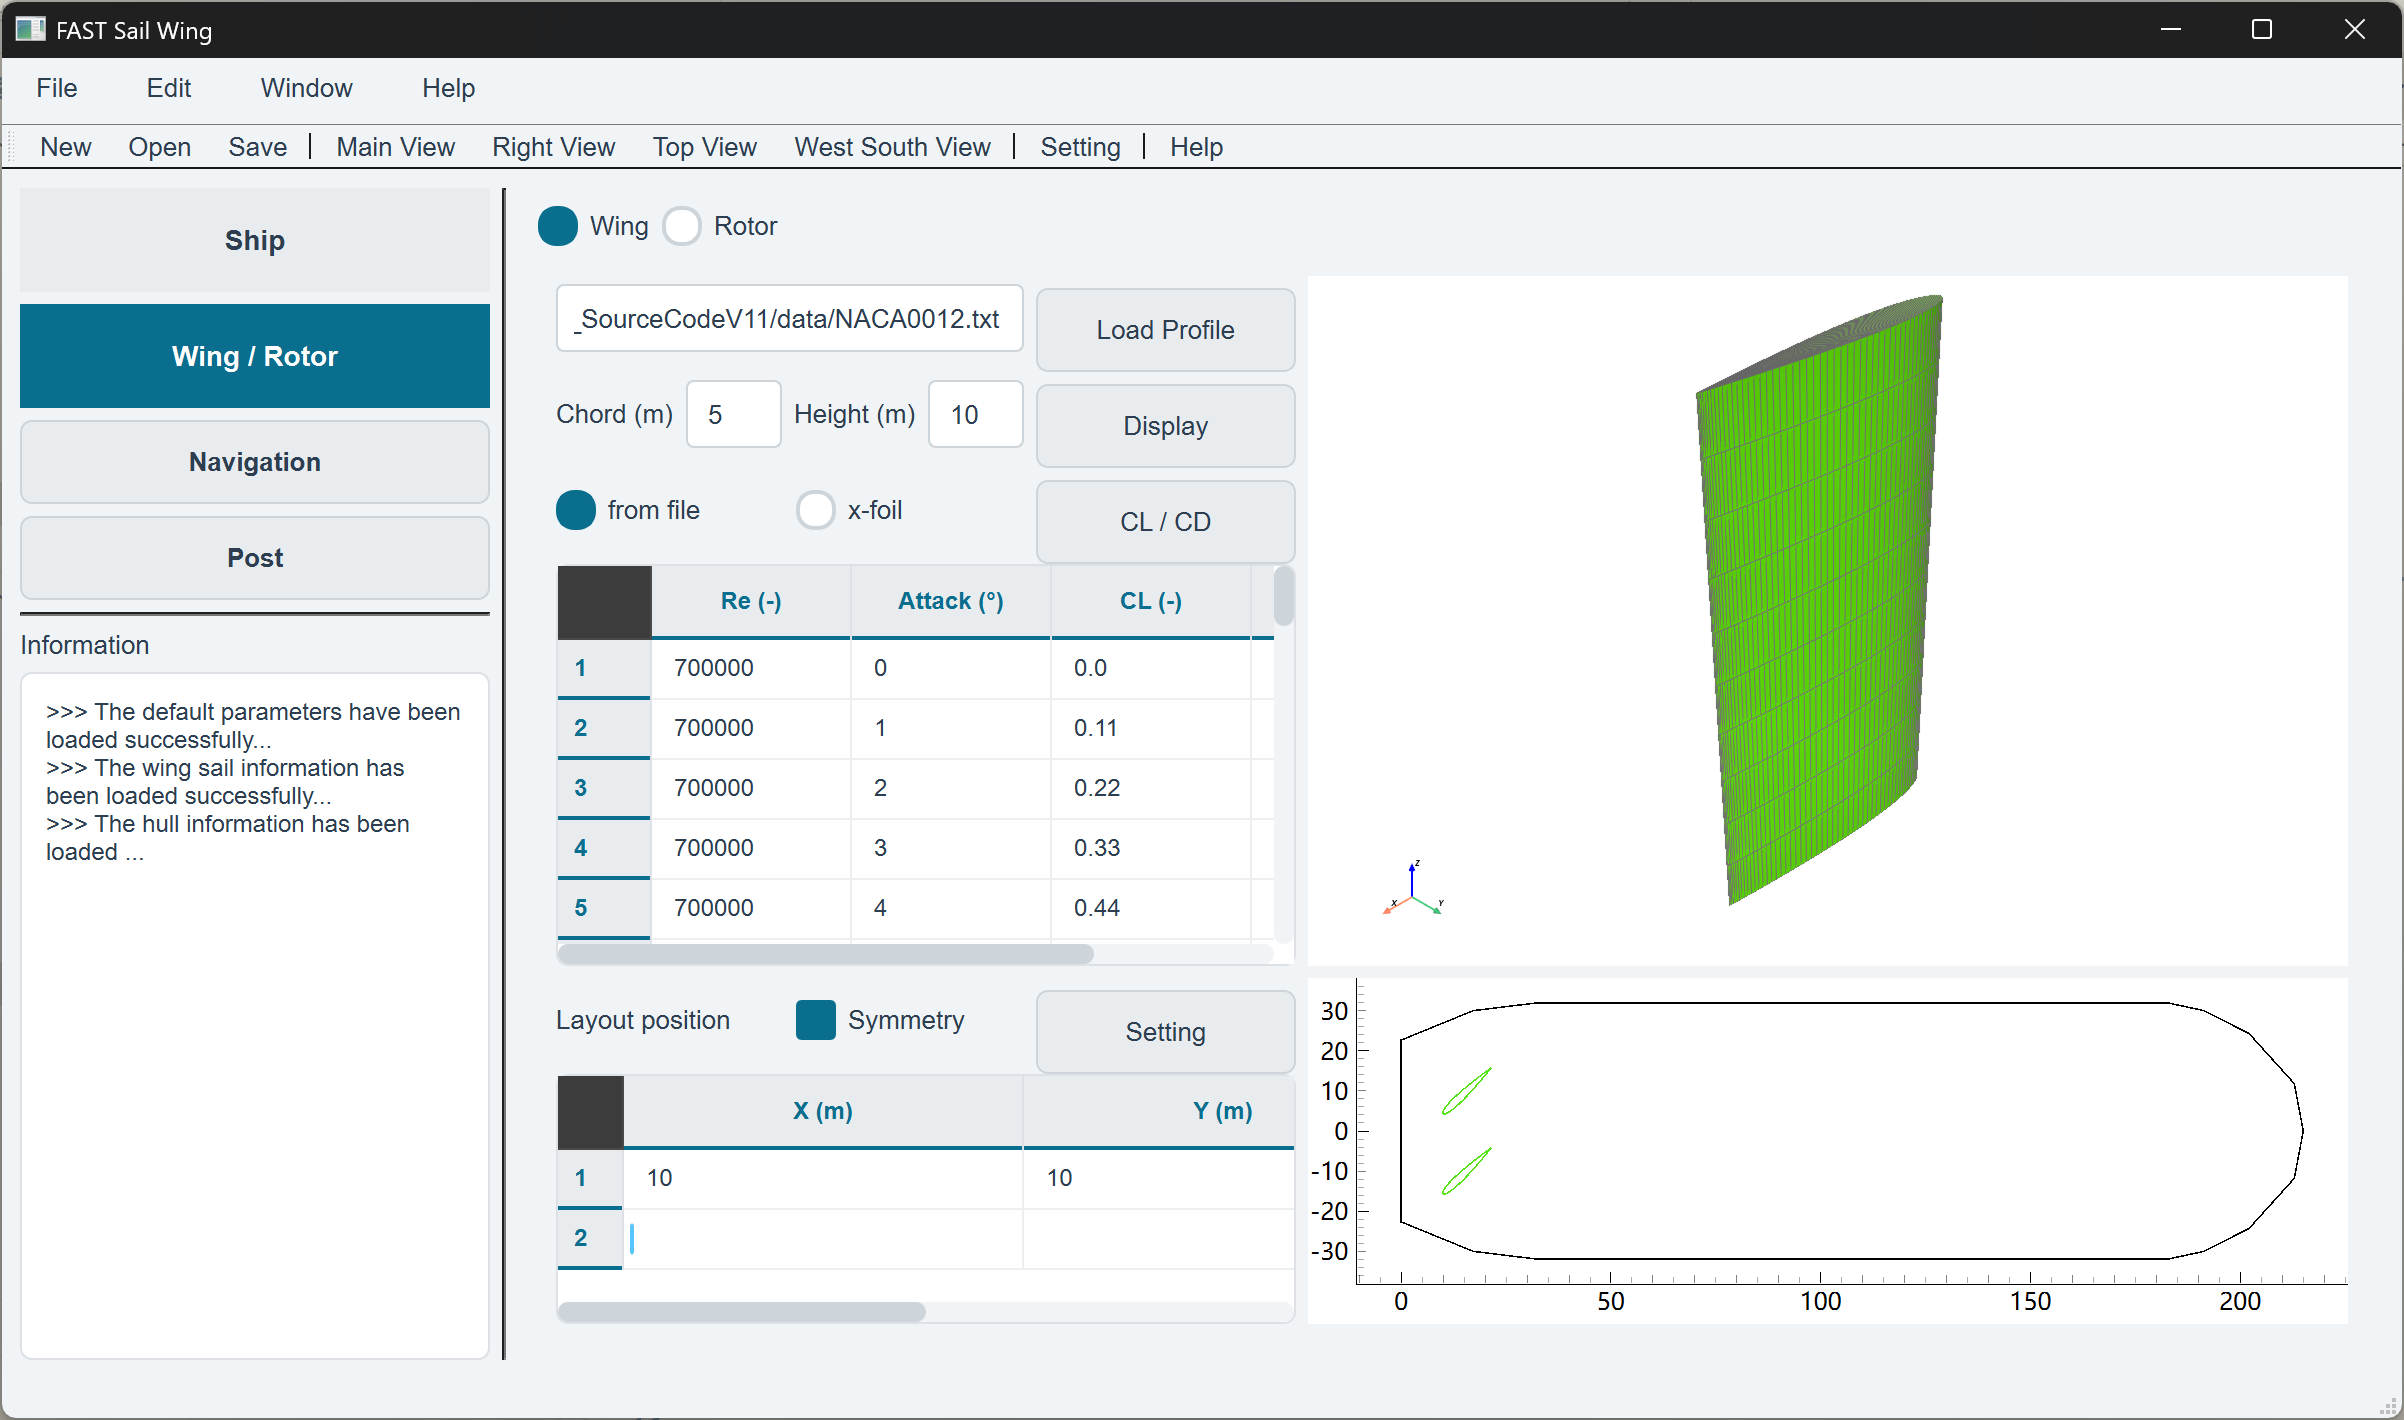
\includegraphics[width=\linewidth]{figures/ui-wing.png}
\par\small （a）翼帆页面
\end{minipage}
\par\medskip
\begin{minipage}{0.95\linewidth}
\centering
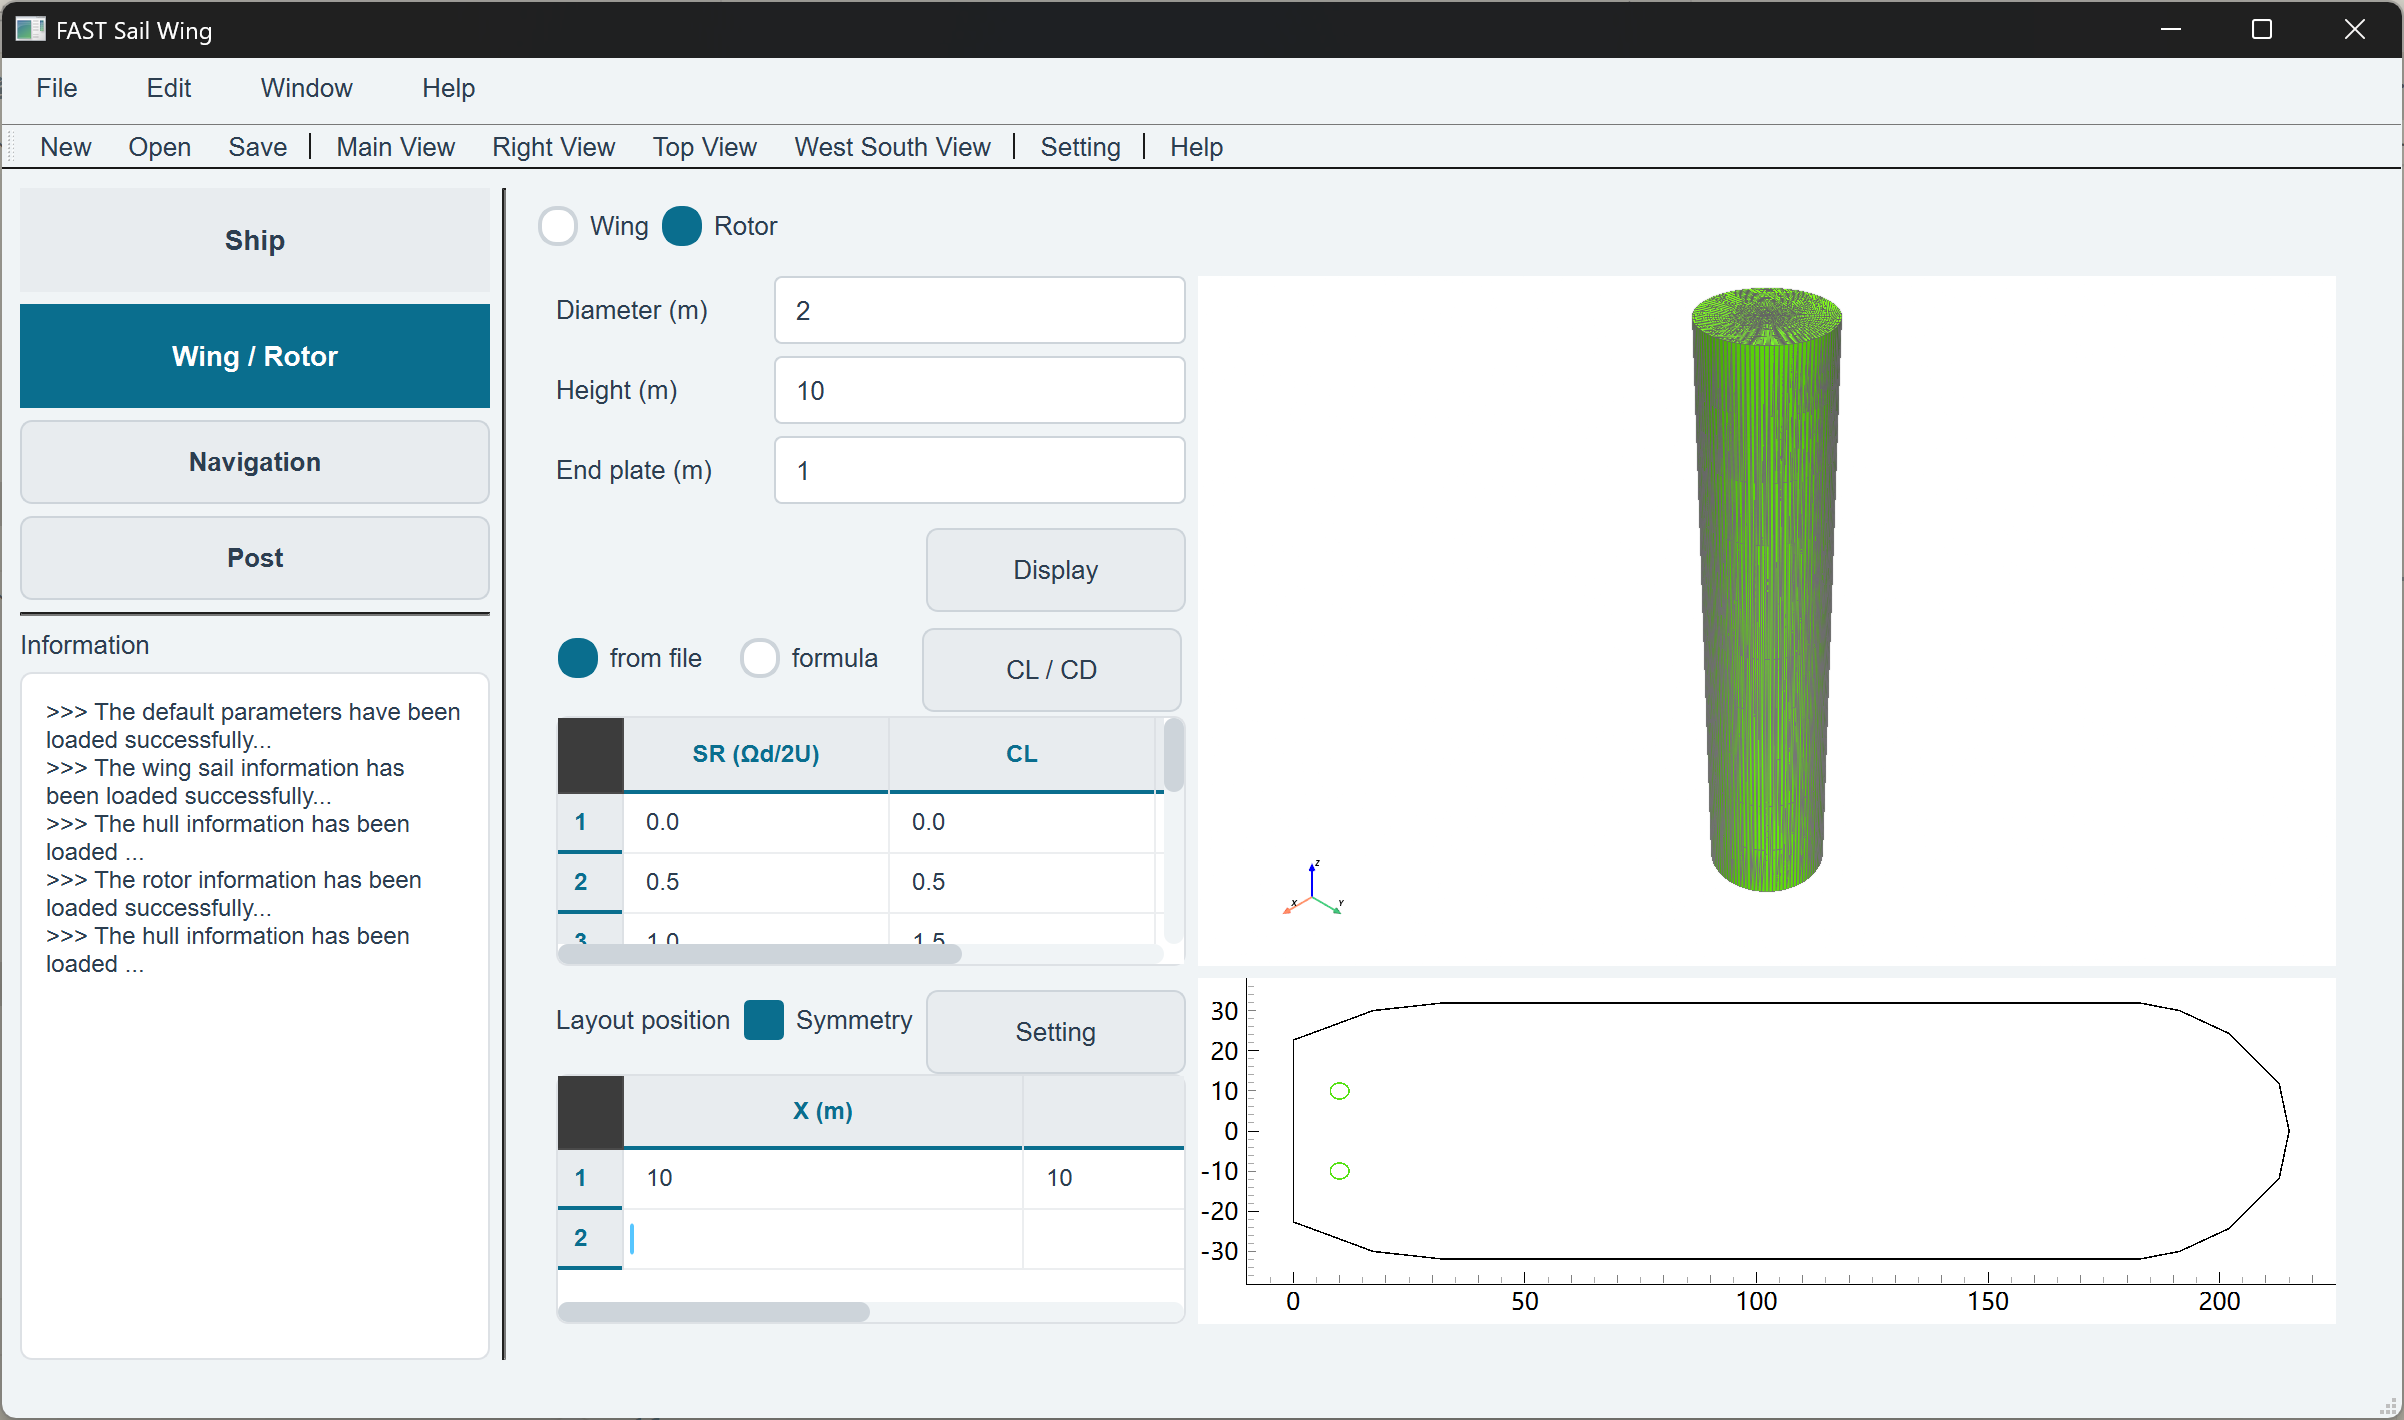
\includegraphics[width=\linewidth]{figures/ui-rotor.png}
\par\small （b）转筒帆页面
\end{minipage}
\caption{翼帆与转筒帆参数及气动性能界面}
\label{fig:ui-sails}
\end{figure}


航线模块读取各航路点的经纬度，并利用相邻航路点计算航段距离和航向。本模块页面见图~\ref{fig:ui-navigation}。风场数据可载入预先利用下载脚本生成的逐航路点 ERA5 航线气象文件。程序将风场矢量与船舶航速矢量合成，得到各航路点的表观风速和风向。载入波浪数据时，程序根据有效波高和船宽估算波浪增阻，并可根据航向与波向应用方向修正；载入海流数据时，海流沿航向的分量用于调整对地航速和航段航行时间。推进功率计算仍采用船舶对水航速。

\begin{figure}[htbp]
\centering
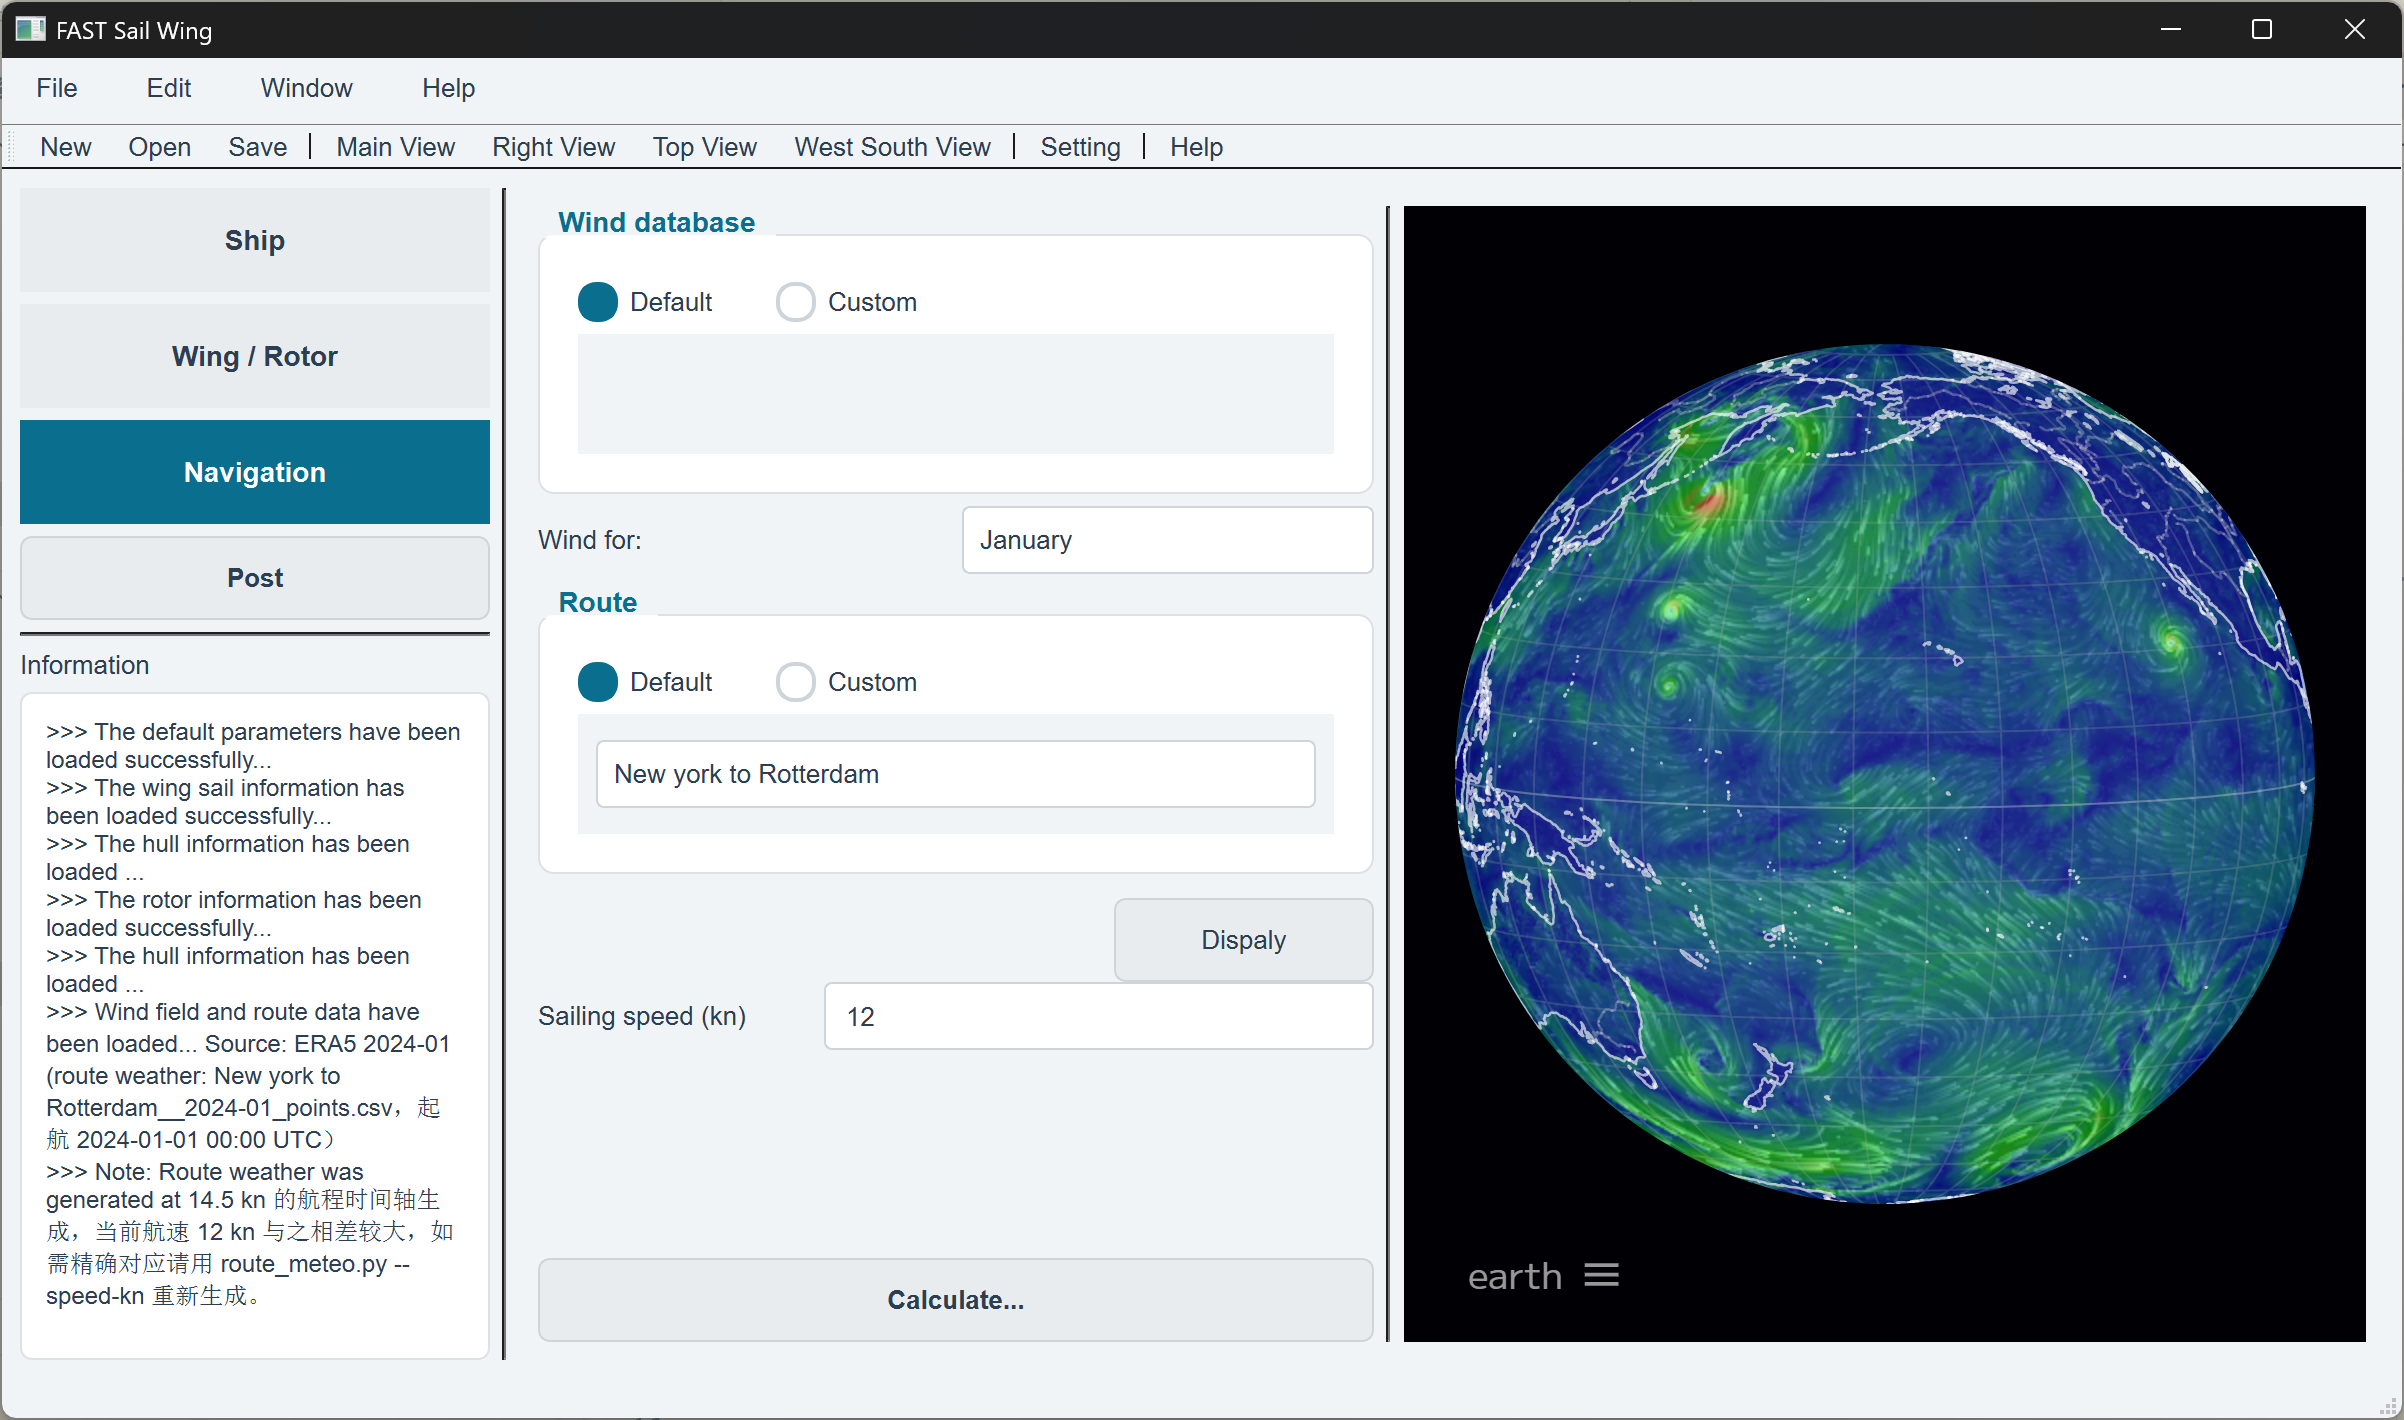
\includegraphics[width=0.95\linewidth]{figures/ui-navigation.png}
\caption{航线气象模块界面}
\label{fig:ui-navigation}
\end{figure}


对于无帆工况，程序以静水阻力为基础；对于有帆工况，程序从船舶阻力中扣除风帆沿航向的助推力。若启用波浪增阻，波浪增阻同时加入两种工况。随后，程序结合伴流分数、推力减额分数、相对旋转效率、螺旋桨直径及螺旋桨静水特性，求解螺旋桨工作点和推进功率。螺旋桨特性数据按线性插值处理。每个航段的推进功率取其两端航路点功率的平均值。

主机燃油消耗由航段推进功率、对应负荷下的主机比油耗和航段航行时间共同确定。程序使用输入的主机标定功率计算负荷率，再从主机油耗率曲线插值得到相应比油耗。航段油耗按“比油耗 × 航段平均功率 × 航段时间”计算并沿航线累加，分别得到无帆和有帆工况的总油耗。海流数据可通过改变航段航行时间影响航次油耗。程序将无帆与有帆总油耗之差作为节油量，并以无帆总油耗为基准计算航次节油率；各航段节油率用于结果曲线展示。航路包含 $N$ 个航路点时，对应 $N-1$ 个航段。

程序还可基于上述主机航次油耗计算单航次 CII 估算值。该功能采用船舶载重吨（DWT）和航程，结合所选燃料的二氧化碳转换系数，分别计算使用风帆前后的航次碳强度。该结果为仅计主机油耗的航次估算，不是 IMO 年度 CII 评级，不包含辅机、锅炉、旋筒驱动耗电及年度评级所需的其他项目。

程序通过输入检查、阻力数据校验、计算结果有效性检查及自动化测试，对模块调用顺序和数值处理进行软件层面的核对。此类检查用于发现输入格式错误、参数缺失、计算范围越界和程序回归问题，并不等同于模型的实船精度验证。计算结果的可靠性取决于船舶阻力、螺旋桨特性、风帆气动力、主机油耗率和环境数据是否与目标船舶及工况相匹配。本文将其定位为给定输入条件下的风帆助推效果估算工具。模型精度仍需通过独立的水池试验、实船功率与油耗记录或其他适用的基准数据进行验证。
\FloatBarrier

\subsection{模型验证与基准工况对比}
\todo{使用试验数据、公开算例或可靠计算结果开展对比，说明误差和适用范围。}

\section{典型航线算例与结果分析}
\subsection{算例船舶、翼帆配置与航线条件}
\todo{列出船舶主尺度、航速、翼帆配置、螺旋桨参数、航线和月份。}
\subsection{沿航线翼帆推力与推进功率变化}
\todo{展示助推力和有帆、无帆功率曲线，解释不同相对风条件下的变化。}
\subsection{航程燃油消耗与节油效果}
\todo{填写总油耗、节油量及节油率，解释主要节油航段。}
\subsection{关键参数影响与模型局限}
\todo{选择航速、月份或翼帆面积中的一至两个变量开展对比，讨论月平均风场、侧向力及其他简化假设的影响。}

\section{结论}
\todo{归纳两至三条由验证和算例支持的结论，说明适用范围及后续改进方向。}

\section*{致谢}
\todo{填写需要致谢的机构或个人；无致谢内容时删除本节。}

% 保留可供正文引用的唯一键；专著采用 [M] 文献类型标识。
\begingroup
\renewcommand{\refname}{参考文献}
\begin{thebibliography}{9}
\renewcommand{\baselinestretch}{1}\songti\fontsize{9pt}{16pt}\selectfont
\setlength{\itemsep}{0pt}\setlength{\parsep}{0pt}
\bibitem{lr2021flettner}
Flettner rotor savings calculator: an interactive tool to determine the potential impact on the net propulsion fuel consumption when operating a Flettner Rotor System[EB/OL]. Lloyd's Register, 2021[2026-10-02]. \url{https://flettner.lr.org/}.
\bibitem{holtrop1982}
HOLTROP J, MENNEN G G J. An approximate power prediction method[J]. International Shipbuilding Progress, 1982, 29(335): 166--170.
\bibitem{holtrop1984}
HOLTROP J. A statistical re-analysis of resistance and propulsion data[J]. International Shipbuilding Progress, 1984, 31(363): 272--276.
\bibitem{harvald1983}
HARVALD S A. Resistance and propulsion of ships[M]. New York: Wiley-Interscience, 1983.
\bibitem{molland2011}
MOLLAND A F, TURNOCK S R, HUDSON D A. Ship resistance and propulsion: practical estimation of propulsive power[M]. Cambridge: Cambridge University Press, 2011.
\bibitem{drela1989}
DRELA M. XFOIL: an analysis and design system for low Reynolds number airfoils[C]//MUELLER T J. Low Reynolds Number Aerodynamics. Berlin, Heidelberg: Springer, 1989. (Lecture Notes in Engineering, Vol. 54).
\bibitem{demarco2016}
DE MARCO A, MANCINI S, PENSA C, et al. Flettner rotor concept for marine applications: a systematic study[J]. International Journal of Rotating Machinery, 2016, 2016: 3458750.
\bibitem{yanyasheng2019}
闫亚胜. 风能在现代船舶风翼助航中应用研究[J]. 海洋工程装备与技术, 2019, 6(S01): 389-394.
\end{thebibliography}
\endgroup

\end{document}
